\documentclass[letterpaper, 10 pt, conference]{ieeeconf}  % Comment this line out if you need a4paper
\IEEEoverridecommandlockouts
\overrideIEEEmargins                                      % Needed to meet printer requirements.

%\usepackage{graphics} % for pdf, bitmapped graphics files
%\usepackage{epsfig} % for postscript graphics files
%\usepackage{mathptmx} % assumes new font selection scheme installed
%\usepackage{times} % assumes new font selection scheme installed
%\usepackage{amsmath} % assumes amsmath package installed
%\usepackage{amssymb}  % assumes amsmath package installed
%\usepackage{amsthm}
%\usepackage[style=ieee]{biblatex}
%\addbibresource{references.bib}
%
%%\theoremstyle{definition}
%%\newtheorem{definition}{Definition}[section]

%\usepackage{amssymb}
%\usepackage{graphicx}
%\usepackage{epstopdf}
%\usepackage{amsmath}
%\usepackage{subfigure}
%\usepackage{multirow}
%\usepackage{pbox}
%\usepackage{algorithm}
%\usepackage{algpseudocode}
%\usepackage{bm}
%\usepackage{url}


%%%%%%

%\documentclass[conference]{IEEEtran}
%
\usepackage{graphicx}
\usepackage{amsmath}
\usepackage{mathrsfs}
\usepackage{array}
\usepackage{enumerate}
\DeclareMathOperator*{\argmin}{arg\,min}
\DeclareMathOperator*{\argmax}{arg\,max}
\usepackage{amssymb}
\usepackage{mathtools}
\usepackage{breqn}
\usepackage{algorithm}
\usepackage{algorithmic}
\usepackage{varwidth}
\usepackage{subcaption}
\newtheorem{lemma}{Lemma}
\makeatletter
\def\BState{\State\hskip-\ALG@thistlm}
\makeatother
\bibliographystyle{ieeetr}


\newcommand\NB[1]{$\spadesuit$\footnote{NB: #1}}
\newcommand\RP[1]{$\clubsuit$\footnote{RP: #1}}

\newcommand*{\Z}{\mathbb{Z}}
\newcommand*{\N}{\mathbb{N}}
% reference package for bibtex

%\usepackage{biblatex}
%\addbibresource{mybibliography.bib}

%\usepackage[
%backend=biber,
%style=numeric,
%sorting=ynt
%]{biblatex}

%\addbibresource{mybibliography.bib}


% correct bad hyphenation here
\hyphenation{op-tical net-works semi-conduc-tor}


\begin{document}
%
% paper title
% Titles are generally capitalized except for words such as a, an, and, as,
% at, but, by, for, in, nor, of, on, or, the, to and up, which are usually
% not capitalized unless they are the first or last word of the title.
% Linebreaks \\ can be used within to get better formatting as desired.
% Do not put math or special symbols in the title.
%\title{Using Hidden Markov Models to Improve Autonomous Vehicle Decision Making - Problem Formulation}
%\title{A Hidden Markov Models-based Approach for Automotive Predictive and Assistive Control}
%\title{\LARGE \bf A Hidden Markov Model-based Approach for Predictive and Assistive Control in Semi-Autonomous Vehicles}
\title{\LARGE \bf A Hidden Markov Model-based Monitor for Predictive and Assistive Control of Hybrid Autonomous Systems}
\author{Rahul Peddi and Nicola Bezzo%
\thanks{Rahul Peddi and Nicola Bezzo are with the Department of Systems and Information Engineering and the Charles L. Brown Department of Electrical and Computer Engineering, University of Virginia, Charlottesville, VA 22904, USA. Email: {\tt \{rp3cy, nb6be\}@virginia.edu}}
%\thanks{$^{2}$Esen Yel is with the Department of Systems and Information Engineering, University of Virginia, Charlottesville, VA 22904, USA. Email: {\tt ey3un@virginia.edu}}
}



%\author{\IEEEauthorblockN{Rahul Peddi$^1$ and Nicola Bezzo$^{1,2}$} 
%\IEEEauthorblockA{
%\small
%$^1$Department of Systems and Information Engineering\\
%\small
%$^2$Department of Electrical and Computer Engineering\\
%\small
%University of Virginia\\
%Email: \{rp3cy, nbezzo\}@virginia.edu}}
%\hyphenation{u-sing}


\maketitle

% As a general rule, do not put math, special symbols or citations
% in the abstract
\begin{abstract}
%\NB{start with Hybrid autonomous systems}
%\NB{abstract needs to be fixed...check my comments below}
%In this work, we develop a monitor that can predict the future states of multiple vehicles within a sensing range, and correct the actions of a user-operated hybrid autonomous vehicle (HAV) to ensure safety. We use a framework that leverages Hidden Markov Model (HMM) theory along with a simplified reachability analysis to perform a risk computation and trust analysis for imminent situations. Our monitor leaves the user in power when safe and intervenes only when the risk is above a threshold, in which case the user action is overwritten by actions that minimize risk. Using this method, we are able to guarantee that the vehicle is safe for the period in which risk is above the threshold. In addition, this approach was validated through simulations of an automotive scenario. \NB{abstract needs to be rewritten}

Hybrid Autonomous Systems have become more commonplace in recent years. These systems
generally consist of a human user sending a command to an autonomous controller, so that
a desired action can take place. Users, however, can pass errant commands that compromise
the integrity or safety of the system. In this paper, we are interested in developing a monitor
that assesses the future risk of the user's actions and leverages the autonomous capabilities to
assist the user. To achieve this, we propose a framework that 
uses Hidden Markov Model(HMM) theory and reachability analysis to predict and estimate with a certain trust the risk of 
future states. In addition, we present a method with which the autonomous controller will correct a user's action.
Finally, we validate the proposed approach with simulations of an automotive setting with moving and stationary obstacles.

%NB{In the abstract we are building a monitor...we need to mention that we leverage HMM, propose a simplified reachability analysis, to predict future states of other surrounding vehicles, compute a risk and, trust to assist a vehicle. We need to mention that the way that }
\end{abstract}
%\NB{abstract should present the problem with a little motivation and the approach with the technique and briefly mention the results}
% no keywords

% For peer review papers, you can put extra information on the cover
% page as needed:
% \ifCLASSOPTIONpeerreview
% \begin{center} \bfseries EDICS Category: 3-BBND \end{center}
% \fi
%
% For peerreview papers, this IEEEtran command inserts a page break and
% creates the second title. It will be ignored for other modes.
\IEEEpeerreviewmaketitle

\section{Introduction}
%\NB{intro needs to be rewritten...follow my comments below}
% no \IEEEPARstart

%\NB{In a not far future, multiple vehicles with different level of autonomy will have to coexist and operate safely. Examples of such vehicles include cars, vessels, aerial vehicles. Different levels of autonomy are available 1 to 5 for cars, hobby  }   

%\NB{Semi-autonomous and autonomous vehicles are finding their way in our society rapidly. Although new advancements in sensing and autonomy are increasing safety by assisting drivers with line changing warning and assisted braking, } 
%\NB{here let's talk about the trolly problem and mention that we see humans as disturbance in this work! discuss about teleoperated robotics that is still big and assistive automation}

In recent years, robotic systems have become more precise and reliable, and as a result they are used in many fields, including military, industry, and even as consumer electronics. For example, aerial vehicles can be used for search and rescue missions or package delivery and intelligent ground vehicles can be used for driving safety or consumer convenience applications. Many of these robotic systems are capable of autonomous behaviors, but the levels of autonomy are varied. For instance, modern consumer vehicles are often equipped with Adaptive Cruise Control (ACC)\cite{acc} or Advanced Driver Assistance (ADA)\cite{adas} capabilities, both of which are systems that have a human in the loop with different levels of involvement. Humans, sometime a pilot or an operator, in remote locations like in military drones operations or behind steering wheels in cars affect the performance, safety, and security of these systems. For aerial vehicles, nearly 33\% of accidents implicate human error \cite{aviacc}. Data from the National Highway Traffic Safety Administration (NHTSA) in 2016 suggests that $94\%$ of crashes on the road are caused by human error \cite{nhtsa}. Of these crashes, $74\%$ are attributed to recognition and decision errors - meaning the user either did not have an understanding of the road conditions or made an unsafe decision. Thus, the human can be often considered as a disturbance in such systems. One solution would be to make every vehicle on the road fully autonomous, without a human in the loop. Full autonomy, however, may not be completely possible for every application, and even if it is the ultimate goal, mixed scenarios (i.e. autonomous and manned vehicles sharing the same road), are inevitable. In this paper, we develop a monitor to assess safety in multi-vehicle operations and propose a switching approach to decide and deploy the correct input and avoid unsafe situations (i.e. collisions).

Although our approach is general for any CPS, we focus on hybrid autonomous systems in which at any time either the user has full control of the vehicle, or the onboard autonomous controller takes over. The propsoed monitor needs to predict what every other vehicle will do, determine the trust of the prediction, predict user's actions consequences, assess their risk, and intervene when needed (i.e. if the risk is very high). We deploy the proposed technique in an automotive case study in which a vehicle is on a road with other vehicles having different behaviors similar to the case depicted in Fig.\ref{fig:hiway}.
%We assume that a user is operating a Hybrid Autonomous Vehicle (HAV), where at any time either the user has full control of the vehicle, or the onboard autonomous controller takes over. This monitor needs to predict what every other vehicle will do, determine the trust of the prediction, predict user's actions consequences, assess their risk, and intervene when needed (i.e. if the risk is very high). 
%In Fig.\ref{fig:hiway}, we show an example of the envisioned desired outcome in an automotive setting. 
In this figure, a user is driving a vehicle (magenta car) behind a slower vehicle (white car). In this case, both actions presented in Fig.\ref{fig:hiway} may appear safe to a driver at the moment, but as can be seen by the red circle, one of the lane changes is considerably riskier in the future, because a rapidly approaching vehicle (blue car) could enter the same space as the user's vehicle (i.e., creating a collision). In this work, we consider the driver's errant actions as a disturbance, and and develop an approach to assist the driver during high risk situations. In order to achieve this goal, we contribute a two-fold approach:
    \begin{itemize}
    \item{a prediction method that can effectively and efficiently estimate the future positions and the risk and trust associated with the predictions of surrounding vehicles} %\NB{and the risk and trust associated with these prediction}
    \item{a switching framework that determines the appropriate the appropriate input to use and the time to switch between user and autonomous behaviors} %\NB{change this. What you mean the severity? }
    \end{itemize}

%\NB{Start this section more general and broad, something like: Modern robotic systems are becoming more precise, they are used in many applications because .... For example aerial vehicles..., cars with different level of autonomy are entering our society....mobile robots used for... Several of these vehicles have different level of autonomy...cars have cruise control, adas, etc... and almost all of them have the human in/on the loop with different levels of involvements. The human, sometime a pilot or an operator in a remote location like in military drones or behind the steering wheel in a car affects the performance, safety, and security of these systems. Here brings some examples about accidents...data from [] show that xx\%of car accidents are due to user/operator errors, in [] xx\% of accidents involving military drones were due to human error....(and so on, show some examples with real data that backup that human is often the problem). Thus, the human is often a disturbance in the system. A solution would be to make everything fully autonomous without human in the loop, however this may not be possible for every application and there going to be always a transition with mixed scenarios (i.e. autonomous and manned vehicles sharing the same road). In this work we develop a monitor (this word should be also in your abstract!!) to assess safety in multi-vehicle operations to avoid unsafe situations (i.e. a collision). For example...explain better Figure 1 here (we may change this figure). Here explain that we are interested in predicting what everybody will do and what a user could do, monitor his actions, assess a risk, build a trust on our prediction, and intervene only if necessary, i.e., ... Our contribution is twofold: ....Although our approach is general for any CPS, we focus on hybrid autonomous systems in which....(explain what is a hybrid autonomous system) and deploy the proposed technique in a case study in which a vehicle is on a road with other vehicles having different behaviors similar to the case depicted in Fig. 1.}
\begin{figure}[h]
    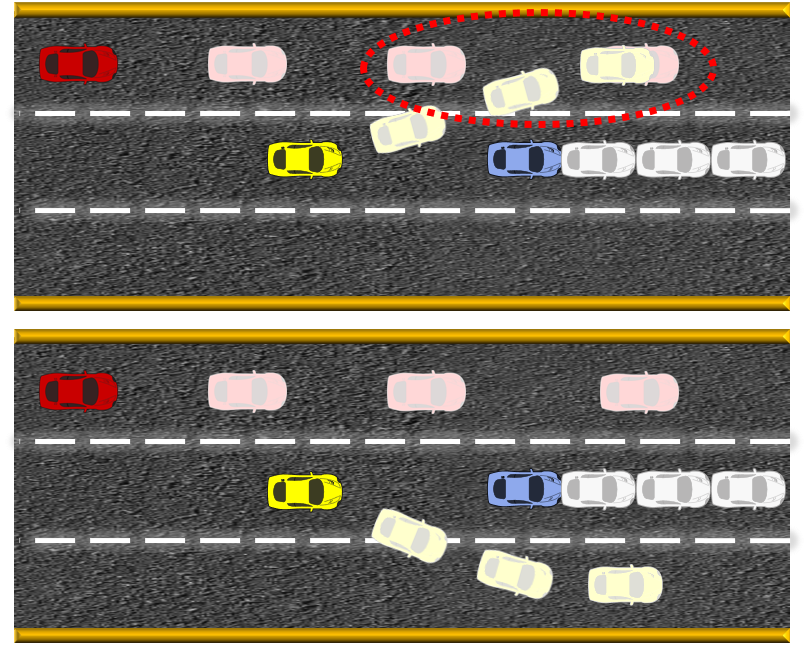
\includegraphics[width=0.48\textwidth]{fig/highway.png}
    \caption{Two possible actions on a highway, where one leads to a dangerous situation in the future(left), and another minimizes risk (right)}
    \label{fig:hiway}
\end{figure}
%\NB{fix this figure. The proportions are off}   
    
    The rest of this paper is organized as follows: in Section \ref{sec:relatedwork}, we discuss related work, and in Section \ref{sec:probform}, we formally define the problem. The general approach is discussed in Section \ref{sec:approach}. In Section \ref{sec:fmwk}, we discuss the specifics of the HMM-based framework, and how it is used to build models. We then use that framework to make online predictions in Section \ref{sec:ahmmpredupdate}, and show how we can fit the models to a system we are observing in Section \ref{sec:omf}. This is followed by a discussion in Section \ref{sec:adapt} on how we use the framework, along with the predictions and fitting, to assist the user. Then we demonstrate our results with MATLAB simulations in Section \ref{sec:sims}. Lastly, we discuss our conclusions and future work in Section \ref{sec:concs}.\NB{fix this part}

    
% You must have at least 2 lines in the paragraph with the drop letter
% (should never be an issue)

\section{Related Work} \label{sec:relatedwork}

The study of semi-autonomous and autonomous vehicles has been growing in recent years. As these options have become more available to the average consumer, driving environments have become more mixed, and researchers approach such environments from different viewpoints; those of improving the knowledge about the environment (i.e. prediction) and those that involve controlling for such environments (i.e. autonomy).

The authors in \cite{mpc} use velocity predictions derived from artificial neural networks and GPS systems for Model Predictive Control (MPC), which is presented as a computationally expensive optimization problem, and the predictions can only be reliably evaluated for one vehicle at a time. The authors in \cite{velnn} and \cite{veldatadriv} take a data science approach and use large data-sets, along with very specific traffic information, in order to make predictions. The use of a Hidden Markov Model based approach for prediction is done in \cite{lanhmm}, where the authors develop an approach treating a vehicle as a hybrid state system to predict the trajectory of a certain behavior. This is done while assuming knowledge of multiple states that cannot be observed from outside. In \cite{woohmm}, motivated by previous work in HMMs, the authors discuss using a simplified form of the hybrid state system with an HMM to improve lane change prediction scalability over multiple vehicles. In our work, we consider the problem of predicting future velocity and when lane changes are expected by leveraging the theories presented in \cite{mpc} and \cite{woohmm}. 

In terms of controlling vehicles in such environments, the authors in \cite{qmdp} use a Point-Based Markov Decision Process (QMDP) to estimate dangerous situations and react with the appropriate autonomous driving behavior in single-lane situations. The QMDP process employs a robust, but computationally expensive value iteration algorithm in order to select the safest action in a single lane situation. In \cite{predcost}, the authors present a prediction and cost-based (PCB) control strategy for autonomous vehicles given a known set of predicted scenarios. In this vein, \cite{vfh+} and \cite{vfh*} discuss reliable obstacle avoidance methods given that obstacle locations and characteristics are known based on artificial physics methods. In \cite{takeover}, with a human-factors based approach, the authors show multiple ways that take-over requests can be generated in partially autonomous vehicles, including performance based and environment based characteristics. In our work, we leverage the idea of sharing control from \cite{takeover}, along with the theories in \cite{vfh*} to control for future unsafe scenarios.

    
\section{Problem Formulation} \label{sec:probform}
 
In this work we are interested in finding an approach to proactively guarantee safety (i.e., something bad will never happen) in multi-vehicle systems operations. We focus on manned vehicles employing an hybrid autonomy scheme as defined in \cite{corke} in which the control authority is shared between the human and the on-board computer. For the sake of brevity we denote this class of vehicles as {\em hybrid autonomous vehicles} (HAVs), In our scheme, the on-board computer is used as a supervisory monitor to predict and assess safety and assist by correcting undesired human behaviors that may lead to unsafe situations and compromise the system's integrity. 

% control in which users may perform undesired actions that can compromise the safety of the entire system 
Formally the problem that we investigate in this work can be stated as: 

\textbf{Problem 1: \textit{Proactive Safe Assisted Planning and Control}:} 
      A hybrid autonomous vehicle (HAV) $h$ is moving in an environment in the presence of other vehicles $q \in R_h(t)$, where $R_h(t)$ is a time varying set of vehicles in sensing/communication range with $h$. The goal is to find a policy to:
    \begin{enumerate}
        \item  predict online other vehicles future states $s$ and their likelihood $p$. Formally, $\forall q \in R_h(t)$:
    \begin{equation}
   S_q=\{{s_q(t), s_q(t+1),..., s_q(t+T)}\}
       \end{equation}
       \begin{equation}
   P_q=\{{p_q(t), p_q(t+1),..., p_q(t+T)}\}
%     \forall q \in R_h(t), S_q=\{{s_q(t), s_q(t+1),..., s_q(t+T)}\}
    \end{equation}
     where $S_q$ is the set of all states, $s_q$, and $P$ is the set of all probabilities, $p_q$ over a finite time horizon $T\in\N$.  
%     assess their likelihood
%    \begin{equation}
%    P=\{{p_q(t), p_q(t+1),..., p_q(t+T)}\}
%    \end{equation}
%    where $P$ represents the set of all probabilities, $p_q(t)$ represents the probabilities at each time, $t$.
    \item assess the risk $0\leq r \leq1$ of a collision during $T$ and
    \item assist and intervene to correct the HAV actions to guarantee safety, i.e., obtain an input policy $U_h=\{{u_h(t), u_h(t+1),..., u_h(t+T)}\}$ such that the risk $r$ is always minimized. 
    \end{enumerate}
   In our specific multi-vehicle case, risk is a function of distance between vehicles. Hence minimizing risk is equivalent to guaranteeing the following:
    
%    surpasses a certain user defined level,$\rho$, we are able to minimize the risk, and guarantee,
    \begin{equation}
        ||{x_h(t)-x_q(t)}|| \geq d_{\textrm{min}}
    \end{equation}
     where $x_h(t)$ and $x_q(t)$ are the positions of the HAV and the $q^{\textrm{th}}$ surrounding vehicle at time $t$ and $d_{min}$ is a minimum safe distance.    
    
    It is important to note that the vehicle that we are assisting is primarily human operated, in the sense that we should intervene only when necessary. %\NB{we are not modifying anything, we are adapting and assisting its operation. This sentence needs to be rewritten.}.
    In other words, unless the HAV has a reachable state that is unsafe, which we define as a situation where $r_h>r_\max$, where $r_\max$ is a user defined threshold, we let the user perform his/her desired actions.

\section{Approach} \label{sec:approach}%\NB{We need to define this section in multiple sections: Offline/Online training; Online Prediction; Online Adaptation}
\begin{figure}[h]
    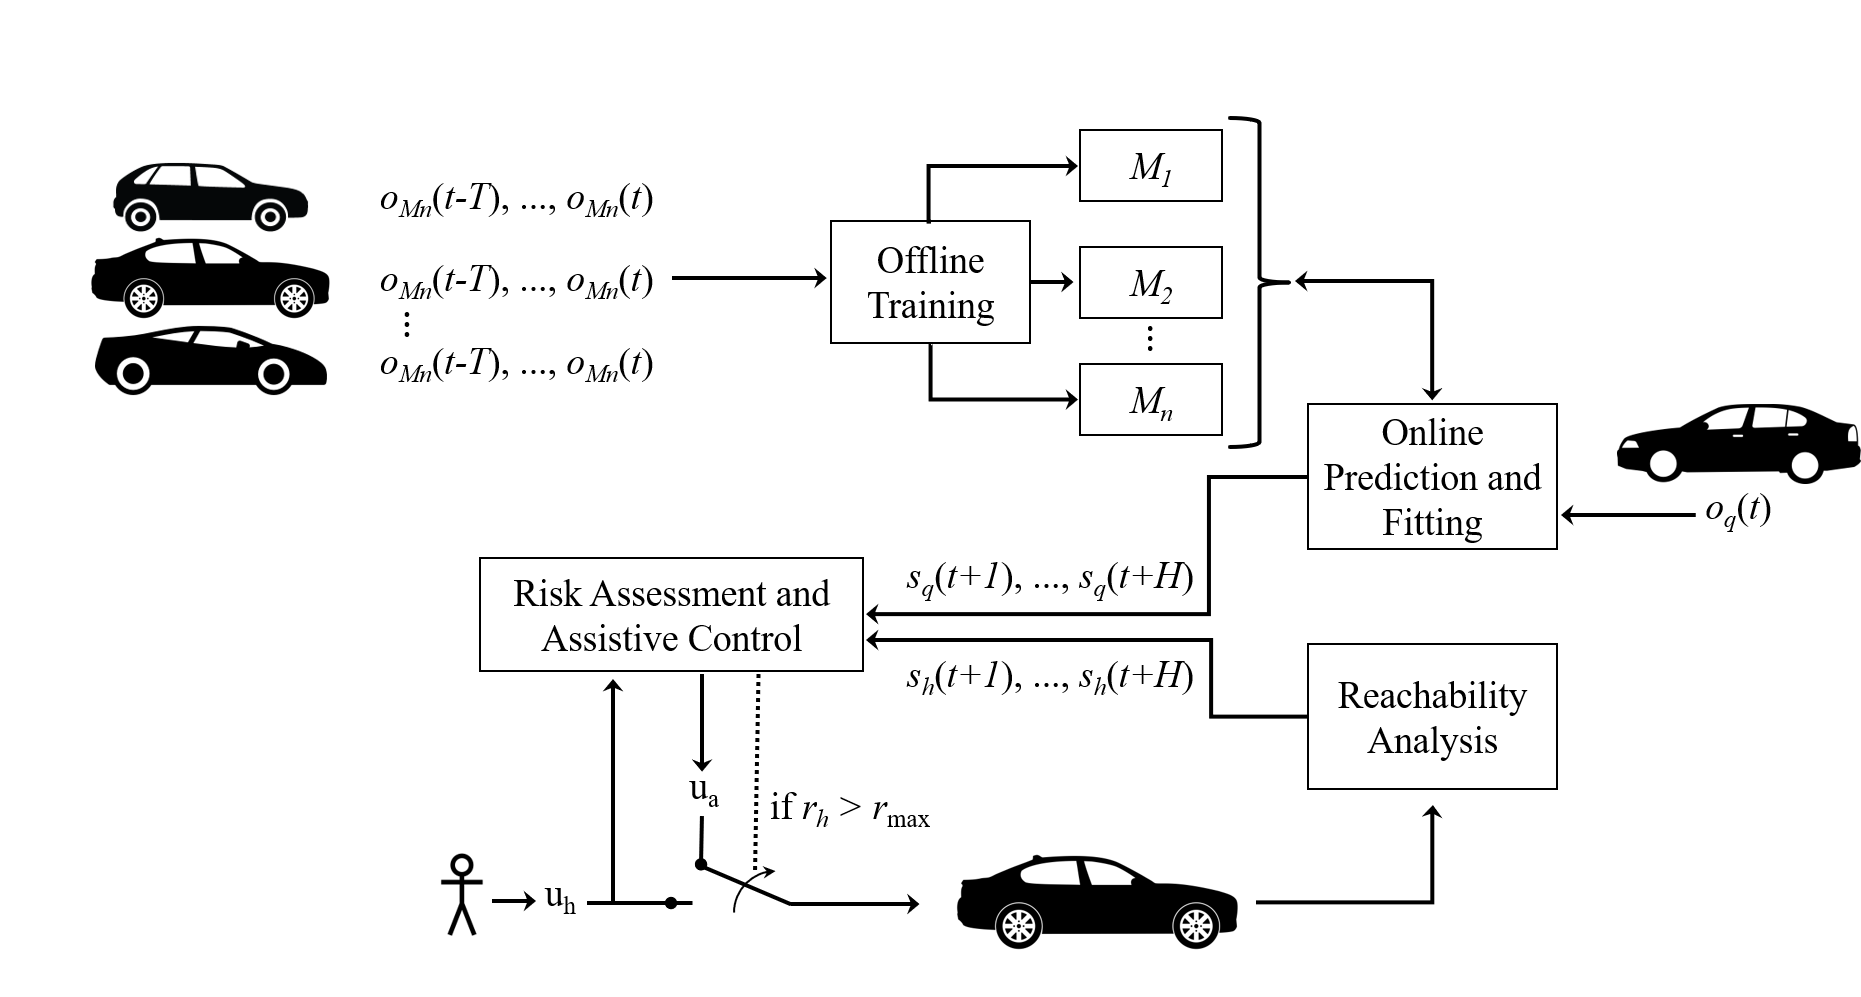
\includegraphics[width=0.48\textwidth]{fig/approach.png}
    \caption{Block Diagram of the Approach}
    \label{fig:app}
\end{figure}
%\NB{fix the lines on this figure}
%\NB{figure is too blurry}
%\NB{that's not a pictorial representation, It's a block diagram.}
%\NB{By using offline training we extract different models representing different vehicle behaviors. These models are then 
%used online to .....}

Our approach is summarized in the architecture presented in Fig.~\ref{fig:app}. We leverage a history of offline observations, $\{o(t-T),\ldots,o(t)\}$, to build different models, $\{M_1,\ldots,M_n\}$, that are then used online to recognize and predict new vehicles' behaviors. Based on these predictions, and the user's input $u_h$, a monitor predicts and assesses whether $h$ could enter any unsafe state. If such an unsafe action is detected, an autonomous control action, $u_a$, is deployed to assist and correct the user's intention. In the next sections, we will go over this framework, explaining in detail each block presented in Fig.~\ref{fig:app}.

%Our approach, shown in Fig.~\ref{fig:app}, has the following components: by using offline training, we extract different models representing different vehicle behaviors. These models are then used online to to predict future states of other vehicles, $\{s_q(t+1),\ldots s_q(t+H)\}$ over a time horizon $H$, thus inferring their behavior to better assess safety and intervene to avoid hazardous situations, like a collision.

%We leverage a history of offline observations, $\{o(t-T),\ldots,o(t)\}$, to build different models, $\{M_1,\ldots,M_n\}$, that are used online to recognize and predict new vehicles' behaviors. Based on these predictions, we want to monitor whether our vehicle, $h$, could enter an unsafe state, based on the user input, $u_h$. If such an unsafe action is detected, an autonomous control action, $u_a$, is deployed to assist and correct the user's intention. In the next sections, we will go over this framework, explaining in detail each block presented in Fig.~\ref{fig:app}.
 
%\NB{be consistent and formal with symbols: variable should be italic, vector should be bold, matrices should be bold upper case etc }
%\NB{fix this}. %\NB{simplify}
 %\NB{this should go in the related work}.% In this work, we train multiple models offline over a horizon $T$, with training sets that capture the behaviors of vehicles \NB{what vehicles...this sentence is incomplete.} \NB{also you are repeating too many times the same thing and always not complete. This section should summarize what we are going to see next: using training data to predict future states and infer the behavior model of other vehicles, compare the prediction with our vehicle prediction to asses safety, monitor and intervene if needed by correcting behavior that can lead to unsafe situations}.
%\NB{In this work we train multiple models offline over an horizon {T}}

\section{HMM-based Training Framework} \label{sec:fmwk}
 In order to predict future states of other vehicles, we perform offline training of data collected over an horizon $T$ to extract and differentiate between multiple behavioral models. To this end, we propose a modified version of the Hidden Markov Model (HMM) \cite{woohmm} which can be described by a tuple $\langle \mathcal{O},\mathcal{S},\mathcal{E},\mathcal{G},\mathcal{P},\mathcal{B} \rangle$  where:
\begin{itemize}
    \item $\mathcal{O}\in\mathbb{R}^T$ is a finite set of observed states $o(t)$ collected over a finite past time horizon $T$, $\mathcal{O} = \{ o(t-T), o(t-T+1), \ldots, o(t)\}$. 
%    In our case $\mathcal{O}$ represent measurements about velocity and positions of surrounding vehicles
    %\NB{change to lower t}.
    \item  $\mathcal{S}\in\mathbb{R}^n$ is a finite set of $n$ unique values that $\mathcal{O}$ can obtain, i.e., $\{s_i,s_j\} \in \mathcal{S} \vert s_i \neq s_j$ with $i\neq j$,and $i,j = 1,\ldots,n$, with $n \in \mathbb{N}$.
    %\NB{no curly brackets when listing counters and indices}
    %\NB{i is equal to OR??? and OR is different to j??? not mathematically correct} The notation $s_{ij}$ represents the state transition from $s_i$ to $s_j$.\NB{there are so many issues in this sentence.}
    \item $\mathcal{C}\in\mathbb{R}^T$ %\NB{what's the dimension of C?}
    is the finite set of emissions, or inferences $c(t)$ that relate to the action taken each state, and $\mathcal{C} = \{ c(t-T), c(t-T+1), \ldots, c(t)\}$. %\NB{what does it mean that it relates to each state? Explain better} $T$, 
    \item $\mathcal{G}\in\mathbb{R}^m$ is a finite set of $m$ unique inferences that $\mathcal{C}$ can obtain. and $g_k \in \mathcal{S}$, where $k = 1,\ldots,m$, with $m \in \mathbb{N}$. 
    \item $\mathcal{P}\in\mathbb{R}^{n\times n}$ is a transition probability matrix. This matrix describes the probability of entering a certain state, $s_{j}$, while currently in a particular state $s_{i}$, denoted as $s_j \to s_i$, defined by:
        \begin{equation}
            p_{ij} = P(s_j\to s_i)
        \end{equation}
        These probabilities are initialized as $1/n$. Each transition probability is calculated by counting the occurrences of each state transition over all transitions from that state:
        \begin{equation} \label{eq:transbuild}
            p_{ij} = N_{ij}/N^*_{i}
        \end{equation}
        where $N_{ij}$ represents the total number of transitions, $s_j \to s_i$, over $T$ and $N^*_{i}$ is the total number of transitions from $s_i$ to any state, and $N_{ij} \leq N^*_{i} \leq T$. The state transition matrix is right-stochastic, meaning the sum of all rows is $1$ and is of the form:
        \begin{equation}
            \mathcal{P} = 
                    \begin{bmatrix}
                        p_{11} & \dots & p_{1n} \\
                        \vdots & \ddots & \\
                        p_{n1} &    & p_{nn}
                    \end{bmatrix}
        \end{equation}
    \item $\mathcal{B}\in\mathbb{R}^{n\times m}$ is the emission matrix, which lists the probability $b_{ik}$ of obtaining emission $g_k$ given state $s_i$:
        \begin{equation} \label{eq:obsref}
            b_{ik} = P(g_k(t+1) \vert s_i(t))
        \end{equation}
        where $i = 1,\ldots,n$. These probabilities are initialized as $1/m$, and are calculated in a similar way to (\ref{eq:transbuild}):
        \begin{equation} \label{eq:obsbuild}
            b_{ik} = N_{g_{ik}}/N^*_{g_{i}}
        \end{equation} 
        where $N_{g_{ik}} \leq N^*_{g_{i}} \leq T$.
        \begin{equation}
            \mathcal{B} = 
                    \begin{bmatrix}
                        b_{11} & \dots & b_{1m} \\
                        \vdots & \ddots & \\
                        b_{n1} &    & b_{nm}
                    \end{bmatrix}
        \end{equation}
 %       The matrices $\mathcal{P}$ and $\mathcal{B}$ will be referenced as ``the parameters" of the AHMM in the rest of this work. \NB{no let's use their name in the paper}
\end{itemize}

This framework is executed over $T$ and a set of parameters is obtained: $\langle \mathcal{P}, \mathcal{B} \rangle$. Our framework is different from a traditional HMM because the states are not hidden, and we know exactly the relationship %\NB{not sure about this and we should not add HMM, We haven't defined it yet and it seems unnecessary to give a name to this unless we have really major changes to the way it computes states and transitions}
%\NB{clarify}
%with implicit parameters $m$ and $n$ \NB{this sentence is confusing}
between states and their corresponding inferences. Because we have all the states and transitions a priori, we can learn the parameters of multiple models offline. %In addition, having the knowledge pertaining to the relationship between states and inferences allows predictions to be made with increased accuracy.\NB{how? This sentence is telling everything and nothing}
The general pictorial representation of the framework is shown in Fig.~\ref{fig:hmm}. %\NB{what's a in the figure?}\NB{figure needs improvement: make it smaller vertically...too much space in between s and c. Increase fonts}.
In this image, nodes labeled $s$ represent the states ($\mathcal{S}$), while those labeled $g$ represent the emissions ($\mathcal{G}$). The lines with the label $p$ are the transition probabilities between states, and those labeled $b$ are the probabilities that each of the connected observations are associated with connected states.
\begin{figure}[h]
    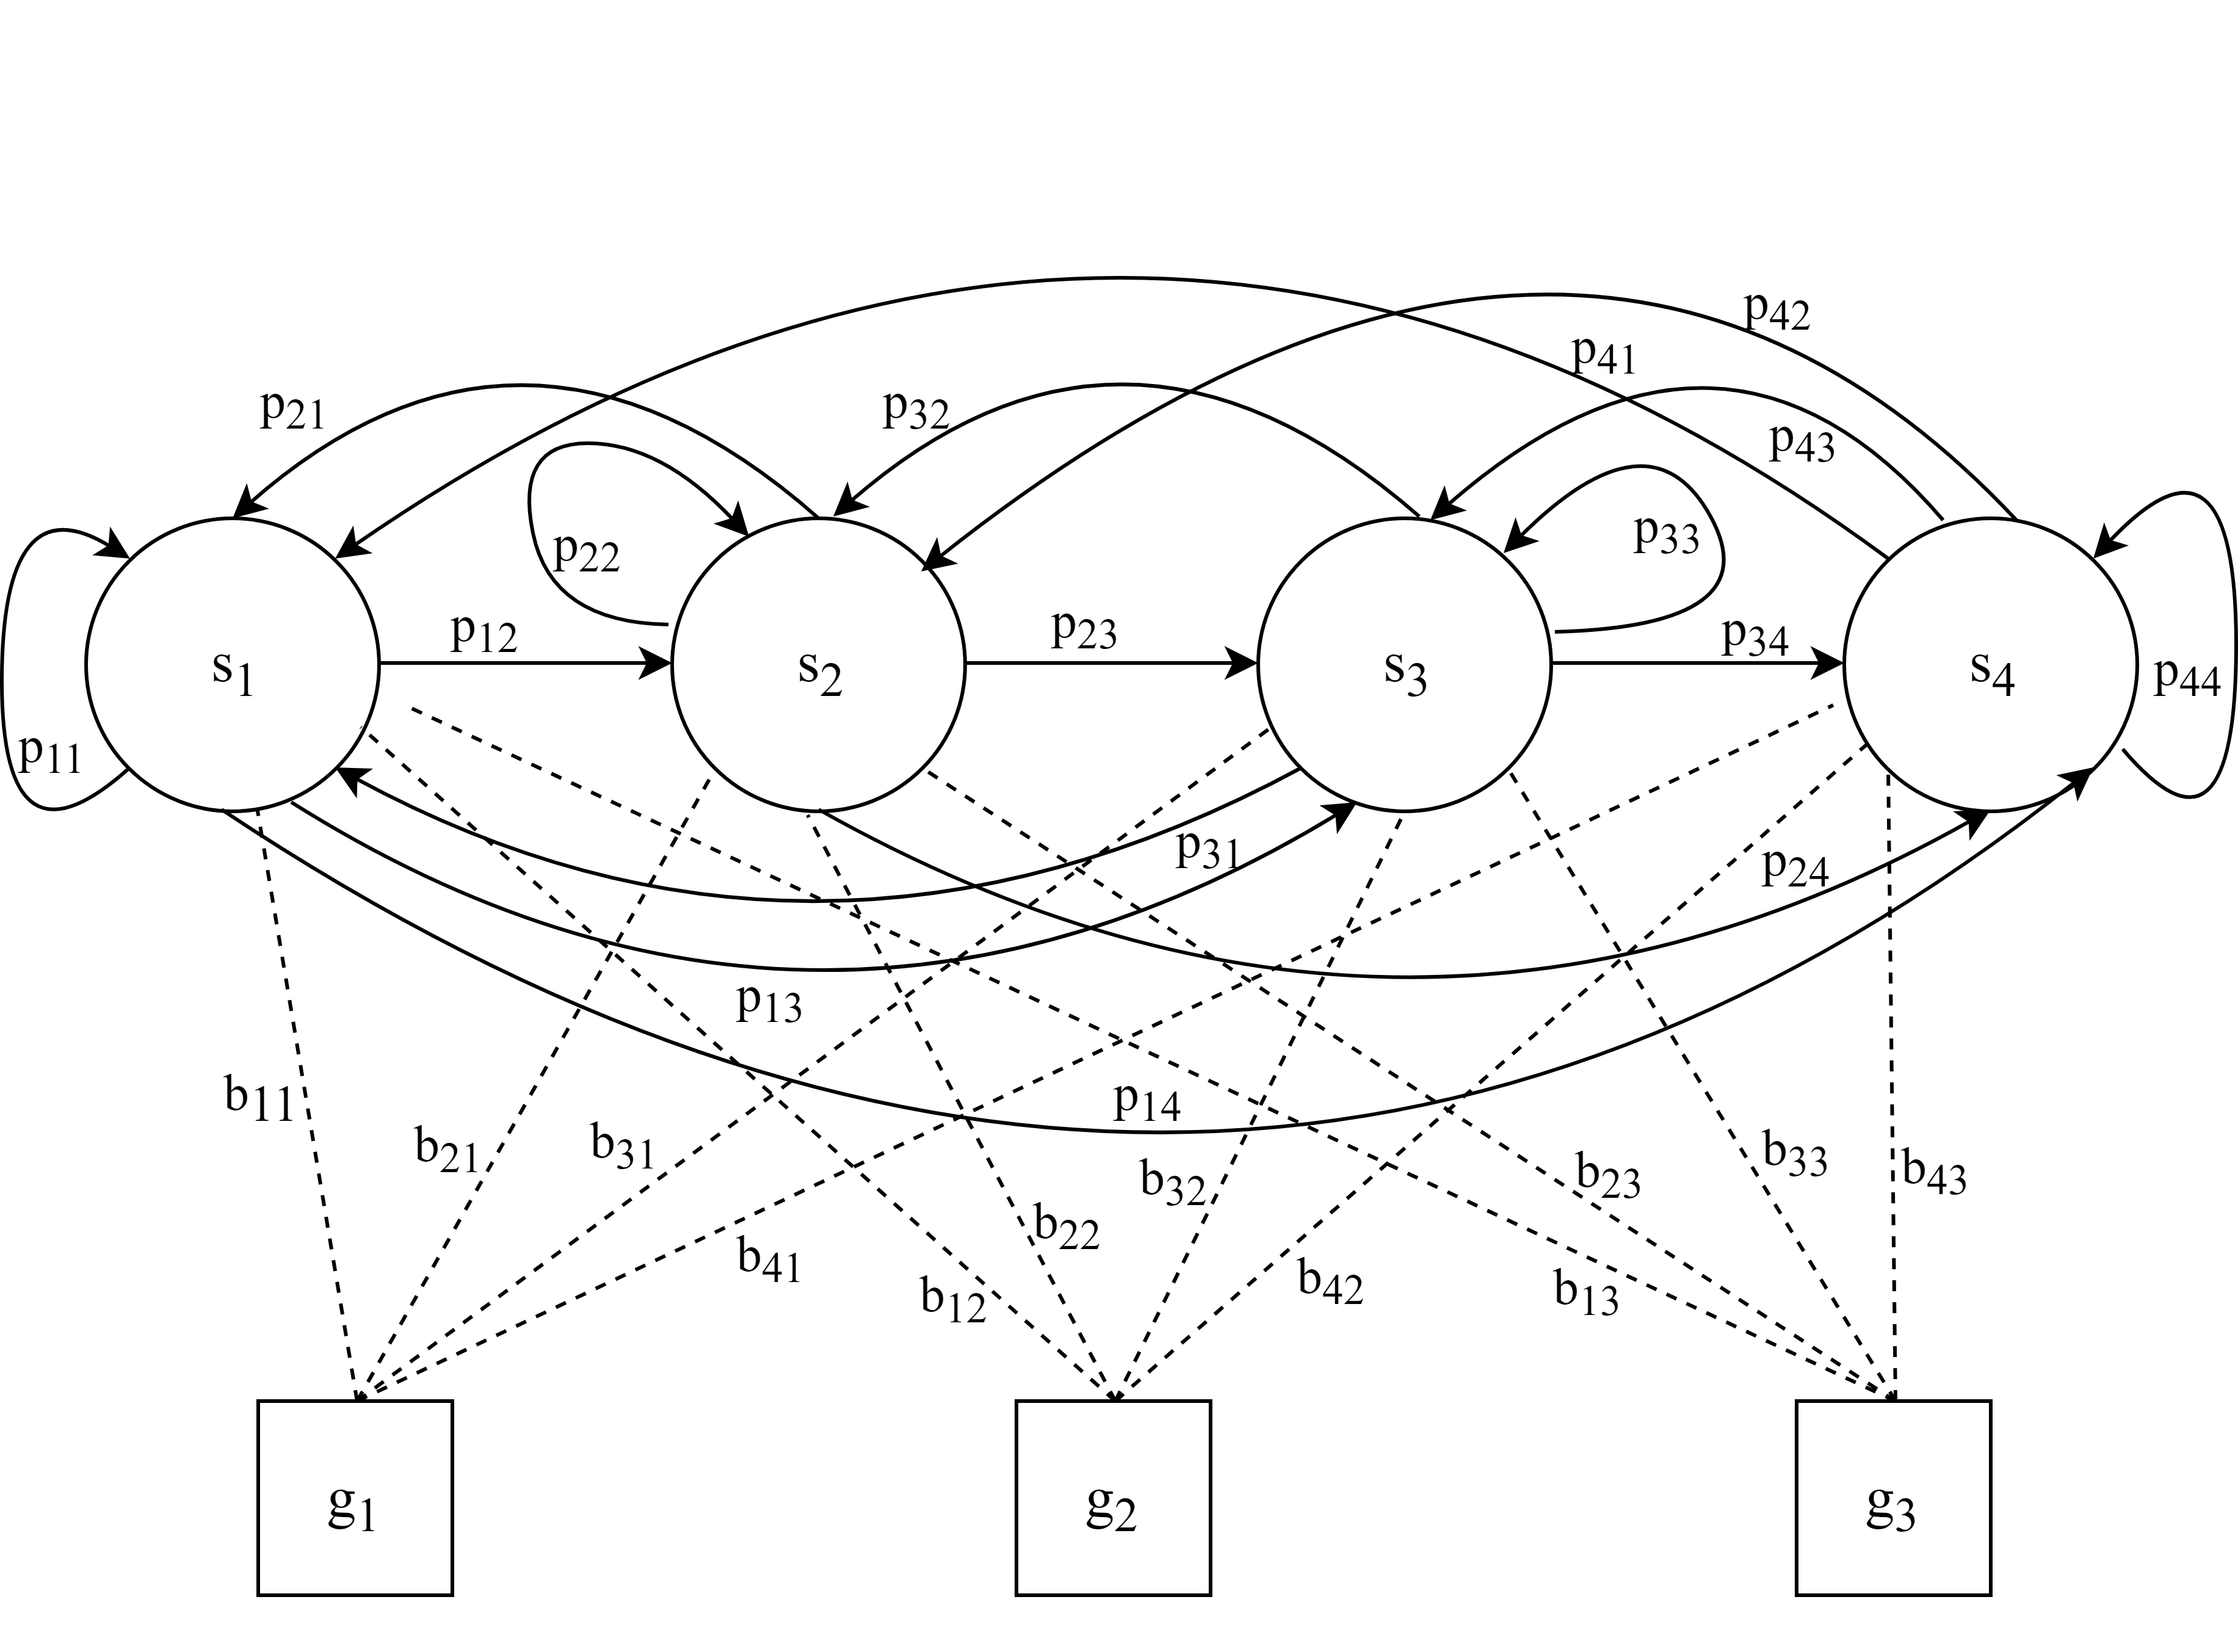
\includegraphics[width=0.48\textwidth]{fig/hmm.png}
    \caption{General Representation of the framework. In this figure, states, emissions, and respective transition and emission probabilities are shown.}
    \label{fig:hmm}
\end{figure}

The specific environment that we are studying involves multiple vehicles that can change their velocities and their lanes.% Within this environment, we implement the framework twice for all of the vehicles, $q$ in our sensing range $R_h$.

Our goal is to predict future velocities $v$ and lanes $l$ of all the surrounding vehicles $q\in R_h$. In this case, $S_v = \{v_1,\ldots, v_n\}$, $S_d = \{d_1,\ldots,d_n\}$, $S_l = \{l_1,\ldots,l_n\}$, where $S_v$ is the set of velocities, $S_d$ is the set of distances between vehicles, and $S_l$ is the set of lanes. The emissions reflect the actions performed between two consecutive states. In our case, emissions are associated the following vehicle input behaviors; changes in velocity and changes in lane. %\RP{Check later} %\NB{let's discuss that these emissions are the inputs that we care i.e., changes in speed and changes in lanes}
For velocity we consider the following 3 emissions,
    
%\NB{too many words...$S_v$ is the set of velocities and $S_d$ the set of distances between vehicles}

\begin{itemize}
    \item[$b_1^v$] {Increasing Velocity if $v(t) > v(t-1)+\delta_v$} 
    \item[$b_2^v$] {Decreasing Velocity if $v(t) < v(t-1)-\delta_v$}
    \item[$b_3^v$] {Maintaining Velocity if $v(t-1)-\delta_v \leq v(t) \leq v(t-1)+\delta_v$}
\end{itemize}
%\NB{formalize...$v(t-1)+\delta_v$ etc}
%\NB{give a name to this emissions...i.e. $b_{1}^v, b_{2}^v$}
%\NB{if not where}
where $\delta_v\in\mathbb{R}^+$ and reflects the change in velocity from one step to another.

For the lanes, the following 3 emissions are considered:

\begin{enumerate}
    \item[$b_1^l$] Changing Left if $l(t) < l(t-1)$
    \item[$b_2^l$] Changing Right if $l(t) > l(t-1)$
    \item[$b_3^1$] Not changing if  $l(t) = l(t-1)$
\end{enumerate}
where we assume that lanes are modeled in increasing order from left to right; i.e. the leftmost lane is $1$ and the rightmost lane is $n$.
%\NB{what does it mean $lane < lane$?}
%\NB{same as before...formalize this}
%\RP{capture that the emission are related to actions}


\section{HMM-Based Online Prediction and Model Updates} \label{sec:ahmmpredupdate} %\NB{perhaps combine with next and add Update in the title}
  Using the framework outlined in Section \ref{sec:fmwk}, given enough observations, we can extract a model for each surrounding vehicle. This model can be used online to predict future states of the system, and this is achieved by collecting more observations online. These online observed states can then be applied to the available, previously collected, emission and transition matrices as lookup tables to obtain the most likely future state. The future state is determined as:
 %\NB{Using the HMM approach outlined in Section...given enough observations, we can extract a model for surround vehicles}. \NB{This model can be used online to predict future states of the system. This is achieved by collecting more observations online. The observed states at time t can then be used in the available emission and transition matrices, as a lookup table, to obtain the most likely next state}At $t$, the parameters of the AHMM can be used to make online predictions about the future states of the observed system. This is done by identifying the current state, $s_{i}(t)$ and applying it to the transition and emission matrices, which are used as lookup tables, to obtain the next most likely state and its likelihood. %We start with the assumption that $\mathcal{P}$ will give conclusive results from which we can predict the future state as follows\NB{remove this}:
%\begin{equation} \label{eq:nextstate}
%    s_{i}(t+1) = \max_{j}[\mathcal{P}_{i(t),j}]
%\end{equation}
%\NB{this equation is wrong. a state is not equal to the probability!}
%There is, however, the possibility that there will be more than one returned states, as the maximum transition probability %can be the same for multiple states. In this situation, we invoke the use of $\mathcal{B}$:
%\begin{equation} \label{eq:nextemis}
%    g_{k}(t+1) = \max_{k}[\mathcal{B}_{i(t),k}]
%\end{equation}
%\NB{this should be only between the two that are uncertain and that formula is not resolving the issue! }
%\NB{equation needed}.
\begin{equation} \label{eq:pred}
   s(t+1) = s_j \in S \vert p_{ij}=\max_p(\mathcal{P}_i)
\end{equation}

In the event that \eqref{eq:pred} returns more than one value, we cross-reference the states with the emission matrix, $\mathcal{B}$ as follows: 
\begin{equation} \label{eq:pred2}
    s(t+1)=s_j\vert g_{ij} = \max_b(\mathcal{B}_i)    
\end{equation}

%\NB{s(t+1) doesn't return multiple values....if there are multiple states that satisfy equation 13. You should go to another line and state that not in an equation environment}
%\NB{change the symbol for and. I'm also not 100\% sure that this expression is correct}
%Because the relationship between states and observations is not hidden, we can use the expected inference, derived from \eqref{eq:pred} to assess which returned state is more accurate \NB{not clear, rewrite}.

In the event that \eqref{eq:pred2} still returns more than one state, we choose the more dangerous transition, which depends on the specific application. For instance, in our case, the more dangerous transition is one that reduces distance between the user's vehicle and other vehicles.
%\NB{go to another line}

Using this approach, we can predict a series of future states over any horizon $H$ by assuming that each prediction for $t+1$ is correct. We re-use the emission and transition matrices to predict a sequence of future states up to horizon $H$.
It is, however, important to note that as $H$ is increased, every successive prediction tends to be less accurate, as the sequence of future predictions is built assuming each of the previous predictions is correct.
%next state at $t+2$ and so on, up to horizon $H$. It is, however, important to note that as $H$ is increased, every successive prediction tends to be less accurate, as the sequence of future predictions is built assuming each of the previous predictions is correct.
%\NB{flip the order} \NB{explain the algorithm}.
Algorithm~\ref{alg:pred} shows how we carry forward this prediction through $H$. In this algorithm, an observed state, $s(t) = s_i$, is used in %\NB{in not with} 
$\mathcal P$ and $\mathcal B$ to find the most likely next state, $s(t+1) = s*_{j}$ %\NB{$s_j^*$}.
At the following step, $s(t+2)$ is calculated using the previously predicted $s_{j^*}$. This process is repeated up to $t+H$, obtaining a series $\{s(t+1),\ldots,s(t+H)\}$ of future states.
%\NB{I think we can remove this if you have explained the procedure well before}
%\NB{assuming that next observation is be the predicted $s(t+1)$}. This process is repeated up to $t+H$.

\begin{algorithm}[ht!]
\caption{Future State Prediction} \label{alg:pred}
\begin{algorithmic}[1]
\WHILE{$t\leq t+H$}
\STATE $s(t) = s_i$
\STATE $s(t+1) = s_j \in S \vert p_{ij}=\max(\mathcal{P}_i)$
\IF{$s_j$ is not a singleton, $s_j\in S$}
\STATE $s(t+1)=s_j\in S\vert p_{ij}=\max(\mathcal{P}_i) \land g_{ij} = \max(\mathcal{B}_i)$
\STATE $s(t+1) \gets s_{j}$
\IF{$s_j$ is not a singleton}
\STATE $s(t+1) = \max_{s_j}S,\forall s_j\in S\vert p_{ij}=\max(\mathcal{P}_i)$
\ENDIF
\ENDIF
\STATE $s_i = s(t+1)$
\STATE $t \gets t+1$
\ENDWHILE
\end{algorithmic}
\end{algorithm}

%\NB{what's $\mathcal{P}_{i}*$? and $j*$...btw it should be $j^*$}
%\NB{this is not correct! The prediction is still not sure because we don't know what's going to happen. On the other hand we want to improve the prediction itself and thus we update the model online}.

It is, however, possible that the online predictions are incorrect, indicating that the offline model does not accurately represent the system we are currently observing. In order to alleviate this issue, $\mathcal{P}$ and $\mathcal{B}$ are updated online. This is achieved by using \eqref{eq:transbuild} and \eqref{eq:obsbuild}, where we adjust $N_{ij}$ and $N_{ik}$, thus also changing $p_{ij}$ and $b_{ij}$. As a result, new transition and emission matrices $\mathcal{P'}$ and $\mathcal{B'}$ are created at each iteration to reflect the updates. In addition, we use a sliding window approach such that the size of the training set is always a constant $T$. %\NB{is always constant $T$}\NB{remove this last part}.
The training set is kept the same size in order to retain computational efficiency and to avoid keeping older and less reliable data. Another option would be to discount older data, however we decide not to use this method in this paper because the transition and emission matrices will grow larger, decreasing the efficiency of the proposed method. 
%$\mathcal{P'}$ and $\mathcal{B'}$ are updated each iteration and will continue to be used for online prediction, making each prediction up-to-date with the online observations. \NB{this last part need to be revised} %\NB{rewrite} %\NB{simplify}

\section{Online Model Fitting}\label{sec:omf}
Using the framework described in Sections \ref{sec:fmwk} and \ref{sec:ahmmpredupdate}, we can extract a model that captures the behavior of a system that we have been observing for $T$. Multiple models $\mathcal{M} = \{M_1,\ldots,M_m\}$ can be extracted using several data sets. Each of these models are characterized by unique transition and emission matrices to capture $m$ different behaviors which will be used at run-time to predict the behavior of any new observed system.
%Multiple models can be extracted using several data sets, and with that we can obtain super-sets containing all the transition and emission matrices for multiple vehicles. These models capture different behaviors. In this work, we assume that models have been collected such that any new system can be fit during run-time. $\mathcal{M} = \{M_1,\ldots,M_m\}$ is the set of $m$ models. %\NB{too many words...M  is the set of m models.}.
The transition and emission matrices of these models are denoted as follows: %\RP{reorder later} %\NB{here we should probably remind the reader that these models capture different behaviors and we assume that we have enough behaviors to model any system during run-time. This concept should be clear also in the introduction}: 
\begin{equation}
    \hat{\mathcal{P}} = \{\mathcal{P}_1,\ldots,\mathcal{P}_m\}
\end{equation}
\begin{equation}
    \hat{\mathcal{B}} = \{\mathcal{B}_1,\ldots,\mathcal{B}_{m}\}
\end{equation}

%\NB{where $M\in\mathbb{N}$ represents the number of models}.

During run-time, we observe new measurements of other vehicles. The challenge here becomes fitting each vehicle's observations to one of the offline models. Until we have enough observations, the prediction may not be accurate. Thus, we need to take into account possible errors in the prediction, $e_i$ as we are matching the vehicle behavior with the offline models. 

%In efforts to minimize situations where transitions are unclear, we propose training multiple models prior to the prediction process.\NB{??? What does this last sentence mean?} \NB{just say that we assume to have collected enough models offline to be able to fit and match any new vehicles that appear in our range}

%\NB{We treat any vehicle observed online as a new system and follow the approach outlined in Section...to obtain P and B. At each iteration P and B are updated and compared with the existing Models. The closest model is chosen to predict the behavior of the system. }Having built multiple models, we observe a new vehicle and begin to execute the framework discussed in Section \ref{sec:fmwk} for two consecutive measurements, $\left[o(t-1),o(t)\right]$. With this information, we are able to further execute the framework and determine parameters $\tilde{\mathcal{P}}$ and $\tilde{\mathcal{B}}$, which stand for the transition and emission matrices for the system we are currently observing. In order to determine the optimal model, we calculate the set of errors, $\hat{e}_{N_{M}} = \{e_{N_1},\ldots,e_{N_M}$\} between our model and each of the offline models:

We treat any vehicle observed online as a new system from which we are interested to compute a model, hence we follow the same procedure in Section \ref{sec:fmwk} to extract transition and emission matrices. Each element of transition matrix, $\tilde{\mathcal{P}}(t)\in\mathbb{R}^{n\times n}$, is initialized to $\tilde{p}_{ij} = 1/n$, where $i,j = 1,\ldots,n$. Similarly each element of the emission matrix,  $\tilde{\mathcal{B}}(t)\in\mathbb{R}^{n\times m}$, is initialized to $\tilde{b}_{ik}= 1/m$, where $i = 1,\ldots,n$ and $k=1,\ldots,m$. At each iteration, these matrices are updated using the method discussed in \ref{sec:ahmmpredupdate}, and are then compared with those of the pretrained models, $\hat{\mathcal{P}}$ and $\hat{\mathcal{B}}$. The most similar model is chosen to predict the behavior of the observed system. To obtain this model, the following error is computed at every iteration:
 %\NB{how are these matrices initialized? We need to show the initial expression of these matrices 1/n ...}
\begin{equation} \label{eq:pnorm}
    \forall{P_i} \in \hat{\mathcal{P}}: e_i = \lVert\tilde{\mathcal{P}}(t)-\mathcal{P}_{i}\rVert_{2}
\end{equation}
%\NB{is it $\hat{e}$ that you are computing? or each element?}
%\NB{check again the expression before; there are a lot of things that are not defined or make little sense}\NB{also I think the l1 and l2 is not correct now. Please check and write the correct expression}
where $\lVert \cdot \rVert_2$ is the $l_2$ matrix norm to return a scalar, which in our case, represents the distance (i.e. error) between transition matrices of the observed model and the offline models. This error indicates the confidence we have in each model. A higher error indicates more uncertainty that our predictions will be correct.

Combining all errors, we obtain $\hat{e} = \{e_1,\ldots,e_m\}$. To make predictions, we select the model $M^*$ with the lowest error: %\NB{What's the l2 of a matrix? Is it a scalar or a vector?}
%\NB{revise this}

\begin{equation}
    M^*=M_i\in\mathcal{M}\vert e_i = \min_e(\hat{e})
\end{equation}
%\NB{need to check variables here}
%\NB{add argmin}
%\NB{i is a index not a model}
%\NB{this is unnecessary. Say this before, above...we find the model $M^*$ that minimizes the error...}
  Given this model, the associates transition and emission matrices, $\mathcal{P}_{i}$ and $\mathcal{B}_{i}$ are used in order to make predictions. The procedure to predict future states is shown in Algorithm~\ref{alg:pred}. In addition to calculating the error, a trust measure for each model is determined:
  \begin{equation}
      \forall e_i \in\hat{e}, \rho_i = 1/e_i
 \end{equation}
 Because trust is inversely proportional to error, the model with the lowest error, $M^*$ also has the highest trust. This trust measure is utilized in Section \ref{sec:adapt} to determine risk.
  
  
  %\NB{something is missing here...we should somehow associate the error to the confidence that we have in that model....bigger errors = more uncertainties. The question becomes what should we do if the error is large or if it is small?? The answer is in the trust. What does it mean to trust more or less?}


%\NB{merge with previous and change to explain better how new data are going to improve your model...}
%If the observed system, however, does not result in an $i^*$ with a low error, the model is updated using the method discussed in Section \ref{sec:ahmmpredupdate} \NB{what does it mean....very confusing}. Because we are attempting to fit the model, rather than build a new one, we have the advantage of having the baseline, the current $N_M^*$ \NB{what is this baseline?}. We are able to leverage the parameters of this model, by  updating $\mathcal{P}_{N_M^*}$ and $\mathcal{B}_{N_M^*}$ as we observe new transitions or make new inferences, much like how we obtain $\mathcal{P}'$ and $\mathcal{B}'$ in Section \ref{sec:ahmmpredupdate} \NB{again very confusing}. In this case, we obtain $\mathcal{P}'_{N_M^*}$ and $\mathcal{B}'_{N_M^*}$. These models can be used to make future predictions using Algorithm \ref{alg:pred}.\NB{this last part is really bad written}


\section{Assistive Control} \label{sec:adapt}


\subsection{Reachability Analysis}

In this work, we are interested in assessing risk of collision. In order to assess this risk we need to predict:
\begin{enumerate}[i.]
\item future states of the surrounding vehicles which are obtained by following the procedure outlined in Section \ref{sec:ahmmpredupdate} and
\item the reachable states of $h$ over a future horizon $H$.
\end{enumerate}
In some of our current work, we are using Hamilton-Jacobi reachability analysis to predict future states of a system under uncertainties \cite{esen}. In this paper, we consider a simplified approach for reachability in which we assume that:
\begin{enumerate}[i.]
\item The vehicle can move to the adjacent lane in one time step $\delta t$ \label{ass:i}
\item future variations of velocity are bounded $v_h-\delta_v \leq v_h\leq v_h+\delta_v$, with $\delta_v>0$ \label{ass:ii}
\end{enumerate}
Both \ref{ass:i}. and \ref{ass:ii}. are worst case scenarios. %Assumption \ref{ass:ii} reflects a physical limitation of vehicles.
Using these assumptions three reachable velocities can be considered as follows:
\begin{enumerate} %\NB{t+1 not i}
    \item $v_h^=(t+1)=v_h(t)$
    \item $v_h^-(t+1)=v_h(t)-\delta_v$
    \item $v_h^+(t+1)=v_h(t)+\delta_v$
\end{enumerate} 
and $\hat{V} = \{v^-(t),v_h^=(t),v^+(t)\}$, which is a time-varying set that depends on the current velocity, $v_h(t)$. Future reachable forward positions can be easily computed as $x_h(t+i)=v(t+i)\delta t$, where $\delta t$ is the sampling time, for each of the three aforementioned velocities. Reachable lanes are modeled as $\hat{L} = \{l_1,\ldots,l_n\}$, in which $n$ lanes are considered. 
%\NB{this set is time varying and depends on the current velocity}
\begin{figure}[ht!]
    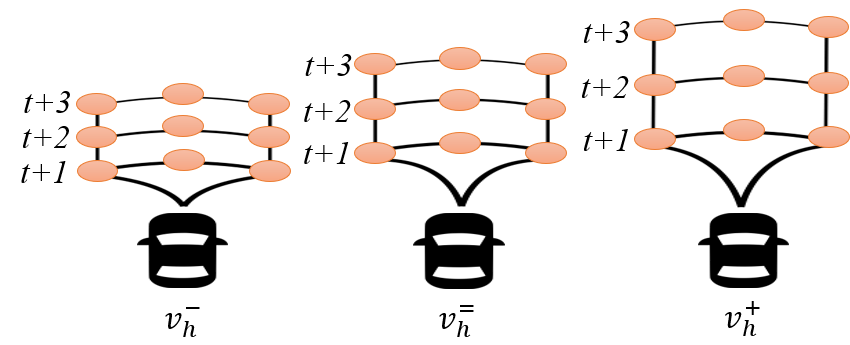
\includegraphics[width=0.48\textwidth]{fig/reach.png}
    \caption{Diagram of each reachable set}
    \label{fig:reach}
\end{figure}
%\NB{the iteration contains?}
Three reachable sets containing all the possible states that can be reached by $h$ are obtained. For example if $h$ is on a 3 lane road and the prediction horizon is 3 time steps, then a total of 27 predictions are obtained, as indicated by the points in Fig. \ref{fig:reach}.
%\RP{dont forget to add picture}
%\RP{Predicting for H allows for trajectory generation for motion planning applications as well}

\subsection{Risk Assessment}

 In this section, we discuss how our framework is used to guarantee safety for an HAV, $h$, over a time horizon $H$.
 
 %\NB{which vehicle? Any?}. In this situation \NB{what situation?}, we have our manned vehicle, $h$, and we have all of the vehicles in our vehicle's sensing range, $R_h$ \NB{$N_{R_h}$ vehicles are in range and can be monitored by $h$ \NB{remember to acknowledge that some vehicles may intermittently enter and exit the range of h}}:
 
 Risk is determined by computing the relative distance between $h$ and all vehicles $q\in R_h$ over the predictive horizon $H$.
 %\NB{and what? What's the solution here? }

%These vehicles will be referred to as agents in the rest of this work \NB{why??? What's wrong with vehicles? Please remove}.

By using the approach presented in Section \ref{sec:ahmmpredupdate}, we can predict future states for all $q$ to obtain:
%\RP{Change to bar or tilde or hat for predictions}
\begin{equation}
    V_q = \{v_q(t+1),\ldots,v_q(t+H)\}
\end{equation}
\begin{equation}
    L_q = \{l_q(t+1),\ldots,l_q(t+h)\}
\end{equation}

%\RP{put in text}

where $V_q$ and $L_q$ are the predicted future velocities and lanes for each vehicle $q$, respectively.
Using these future velocities, we can calculate the positions of each $q$ over the horizon $H$ as $x_q(t) = v_q(t)\delta t$ and obtain the predicted future positions:
\begin{equation}
    \hat{x}_q = \{x_q(t+1),\ldots,x_q(t+H)\}
\end{equation}
We can then calculate relative distance as
\begin{equation}
    \forall q \in R_h: d_q(t) = \lVert x_h(t)-x_q(t)\rVert_2
\end{equation}

%Generating and using the optimal model for each vehicle $q$, as discussed in Section \ref{sec:omf}, we are able to predict where an agent will be in the environment for the user-defined time horizon, $H$, as discussed in Section \ref{sec:ahmmpredupdate}\NB{this sentence is confusing: By using the prediction approach presented in Section...we can predict future states for $q$ over an finite horizon $H$. }. This time horizon defines how far ahead the user wants the system to check, in order to intervene \NB{remove}. A sequence of future states for agent $q$, both in terms of velocity and lateral position, are developed for $H$ using the AHMM parameters and Algorithm \ref{alg:pred} \NB{merge this with the previous section}. Given a sequence of future predicted velocities,


%In this case, we also assume that the driver will continue the behavior he/she is doing at $t$ up to $t+H$. With this assumption, we are able to the estimate the future positions of $h$, obtaining the set:
%\begin{equation}
%    x_h^p = \{x_h(t+1),\ldots,x_h(t+H)\}
%\end{equation}

%\RP{Simplify - Risk is a function of D as follows}
where $\rVert \cdot \lVert_2$ indicates the $l_2$ vector norm. Risk is inversely proportional to distance $d_q(t)$, lane separation $l_q(t)$, trust $\rho$. Specifically the risk $r_q^l(t)$ associated with vehicle $q$ and lane $l$ at time $t$ is computed as follows: %\NB{what about the lanes?}

\begin{equation} \label{eq:riskcalc}
    r_{q}^{l}(t) =
    \begin{cases}
    \frac{1}{d_{q}(t)\rho^*},  & \text{if } l_h=l_q \text{ and } d_{q}(t) > 1  \\
    \frac{1}{\xi d_{q}(t)\rho^*},  & \text{if } l_h\neq l_q \text{ and } d_{q}(t) > 1  \\
        1,                     & \text{otherwise}  
    \end{cases}
\end{equation}

where $\xi$ is the difference in lanes between $h$ and a $q$.
% \NB{what is this function?} 
 The values obtained from \eqref{eq:riskcalc} are calculated for each reachable velocity and position of $h$. For each $q$ and $v$ we can compute the following risk matrix: %\NB{the vehicle are arranged as follows?}:
\begin{equation} \label{eq:riskmat}
\mathcal{R}_{q}^{v}=
\begin{bmatrix}
r_q^{l_1}(t+1)  \dots  r_q^{l_n}(t+1) \\
\vdots  \ddots  \\
r_q^{l_1}(t+H)  \dots   r_q^{l_n}(t+H)
\end{bmatrix} q = 1,\ldots,m,v\in\hat{V}
\end{equation}
%\NB{what you mean interfering?}
Combining together all of the risk matrices we obtain the following superset $\mathcal{R}$:

\begin{equation} \label{eq:superrisk}
\mathcal{R} =
\begin{bmatrix}
\mathcal{R}_{1}^{v_h^-} & \ldots & \mathcal{R}_{m}^{v_h^-} \\
\mathcal{R}_{1}^{v_h^=} & \ldots & \mathcal{R}_{m}^{v_h^=} \\
\mathcal{R}_{1}^{v_h^+} & \ldots   & \mathcal{R}_{m}^{v_h^+}
\end{bmatrix}
\end{equation}
The representation in \eqref{eq:superrisk} suggests that multiple vehicles affect risk in our analysis. We are most concerned with the highest risk at each reachable point, which can be due to any vehicle, and is evaluated as follows: %\NB{any reachable point shown in Fig.}.
\begin{equation} \label{eq:riskdistribution}
 \hat{\mathcal{R}}(i,j) = \max\begin{pmatrix}
 \begin{bmatrix}
\mathcal{R}_{1}^{v^-}(i,j) & \ldots & \mathcal{R}_{m}^{v^-}(i,j) \\
\mathcal{R}_{1}^{v_h}(i,j) & \ldots & \mathcal{R}_{m}^{v_h}(i,j) \\
\mathcal{R}_{1}^{v^+}(i,j) & \ldots   & \mathcal{R}_{m}^{v^+}(i,j)
\end{bmatrix}\end{pmatrix}
\end{equation}
%\NB{what's L? Define every variable, vector, set, etc...be careful that you may have already defined this before in another way}

%\NB{$\hat{r}_{v_h}$ is one value if I have to look this expression. why???}
 where $i = 1,\ldots,H$, $j = 1,\ldots,n$, and $\hat{\mathcal{R}} \in \mathbb{R}^{H\times n}$.
 
 %Using \eqref{eq:lanerisk}, we obtain a distribution of all of the highest risk values for velocity $v_h$. % \NB{how are you combining these risks in one risk?}. 
 In Fig.~\ref{fig:distr}, we show an example of a risk distribution (i.e. $\hat{\mathcal{R}}$), over $H=3$ for velocity $v_h$. The road scenario (Fig.~\ref{fig:roads}) shows the user's vehicle as well as reachable points for the vehicle, as indicated by the lines labeled with timesteps. In addition, other vehicles and future predictions of those vehicles for horizon $H=3$ are also shown in the road scenario.

\begin{figure}[H]
\centering
\begin{subfigure}{.54\linewidth}
  \centering
  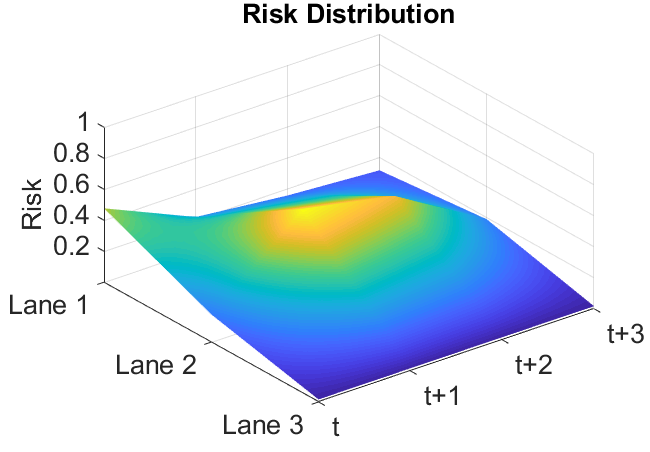
\includegraphics[width=\linewidth]{fig/assist_rd.png}
  \caption{Risk Distribution}
  \label{fig:distr}
\end{subfigure}%
\begin{subfigure}{.46\linewidth}
  \centering
  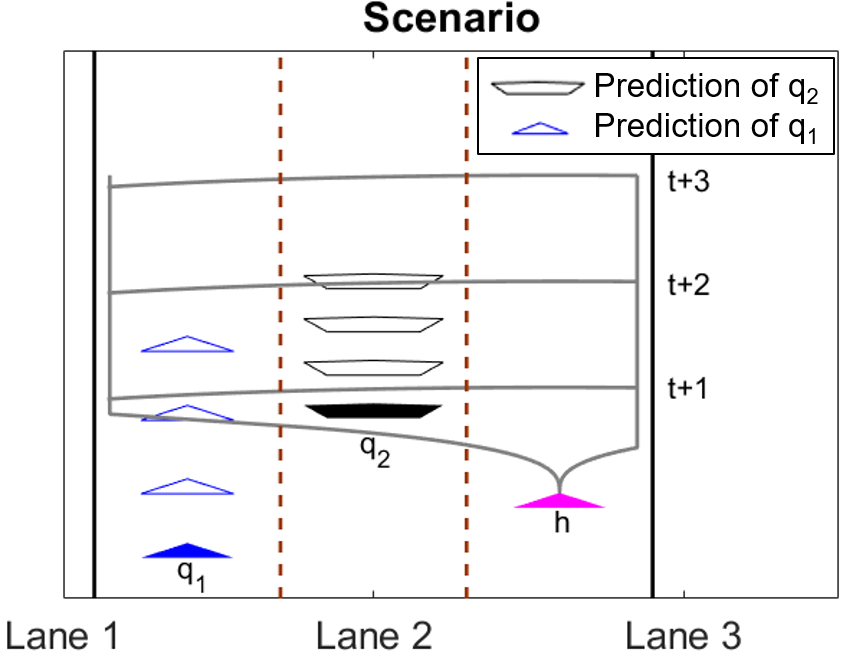
\includegraphics[width=\linewidth]{fig/riskdist_rs.png}
  \caption{Road Scenario}
  \label{fig:roads}
\end{subfigure}
\caption{Risk Distribution and Associated Road Scenario}
\label{fig:riskd}
\end{figure}
%\NB{where is the legend?}

%\begin{figure}[ht]
%    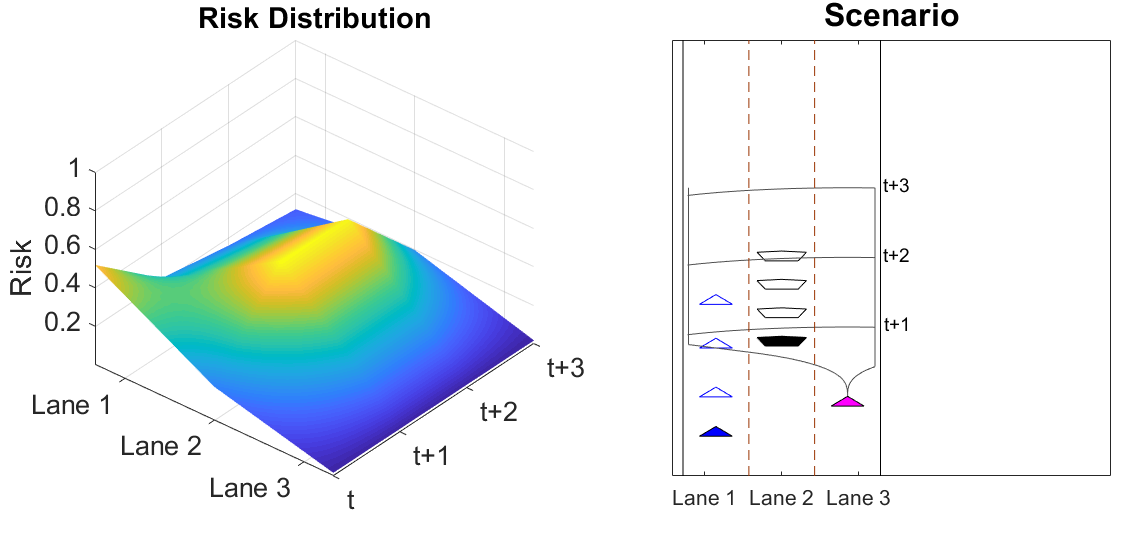
\includegraphics[width=0.48\textwidth]{fig/assist2.png}
%    \caption{The distribution of risk at $v_h$ with $H = 3$ (left) for a certain road scenario (right). The magenta shape is the user's HAV, while the blue and black shapes are the actual positions of other vehicles on the road. Unshaded/outline shapes are predictions for vehicles in successive order; $[t+1,t+H]$.}
%    \label{fig:riskd}
%\end{figure}
%\NB{as mentioned during last meeting use solid filled shapes to show the current position and empty shape (not necessary to have a dashed line) for future states. No need to paint future states with different colors, just use the same color that you used to paint the shape of the vehicle. i.e., if the car on your left is blue, the future states are also blue}
%\NB{avoid this notation, this what?}
%\begin{equation}
%    \hat{\mathcal{R}} = \{\hat{r}^{L},\hat{r}^{C},\hat{r}^{R}\}
%\end{equation}
%\NB{this doesn't say too much. We can remove it probably}
\subsection{Adaptive User Assistance}

%\NB{define dangerous condition}
%\NB{...we propose a policy...}

Given the risk distribution, we can assist our user's potentially unsafe actions to guarantee safety, by performing actions that minimize risk. In order to adapt, we need to first identify whether these actions are going to result in a dangerous situation i.e., a collision. User actions, in this case, are limited to selecting a reachable lane and velocity,
\begin{equation}
u_h = (l_h,v_h), \text{ where } l\in\hat{L}, v_h\in\hat{V}
\end{equation}
A user-set threshold, $r_\max$ is defined. If risk is below $r_max$, we let the user continue his/her desired actions, and if it is above $r_\max$, the autonomous component in the HAV takes control of the system. Given $r_\max$ and the values in the risk distribution, as indicated in Figs.~\ref{fig:reach} and \ref{fig:riskd}, the input $u$ is either the user input $u_h$ or the autonomous input $u_a$ as follows:
% \NB{what does it mean? A limit for risk for what? Be clear}.
\begin{equation} \label{eq:inputctrl}
    u = \begin{cases}
    u_h & \text{ if } \hat{\mathcal{R}}(i,j) < r_\max, \forall\hat{\mathcal{R}}(i,j)\in\hat{\mathcal{R}} \\
    u_a & \text{ if } \exists~\hat{\mathcal{R}}(i,j) >= r_\max
    \end{cases}
\end{equation}
%\NB{this is not what we are implementing...you are looking if any risk between now and H is above the maximum: if yes you switch to autonomous and send the vehicle toward the lane and velocity with the minimum risk associated}
%\NB{we need to define what are the inputs in our system}
%\NB{super confusing. You should simply say that the input $u$ is going to be either the user input or the autonomous input as follows...and then show the equation above.}. 
During run-time, we are monitoring $\hat{\mathcal{R}}$ to find the appropriate pair of actions (velocity and lane) for time $t+1$ that minimize risk. In order to identify the safest actions, we use gradient descent on the risk distribution:
\begin{equation} \label{eq:optpt}
  r^* = \min\{\hat{\mathcal{R}}(1,1),\ldots,\hat{\mathcal{R}}(1,n)\}  
\end{equation}
In other words, we are only concerned with the first row of $\hat{\mathcal{R}}$, which corresponds to $t+1$.
The value $r^*$ gives information about the safest lane to enter and the safest velocity to reach. The optimal input pair can be obtained as follows, $\hat{\mathcal{R}}$:
\begin{align} \label{eq:optpair}
    l^* &=  l_j\in\hat{L}\vert r^* = \hat{\mathcal{R}}(1,j)\in\hat{\mathcal{R}} \nonumber \\
    v^* &=  v\in\hat{V}\vert r^* = \hat{\mathcal{R}}(1,j)\in\hat{\mathcal{R}}
\end{align}
%\NB{so you pick the lane of the minimum risk even if the minimum risk is on t=3?} %\NB{you should pick the lane such that the risk on that lane and for the next iteration is minimized.}
%\NB{what is the dimension of $\hat{r}_q^l$? From (22) it's one value} \NB{Why argmin with respect to $l_i$ and not $l$? Is it just $l_i$?}\NB{this expression is not correct! You need to pick the l and v associated to the minimum risk!}

%\NB{what do you mean that you are picking $v_h$? What about if you have $v_h^-$ that is the best one?}
%\NB{what do you mean that you pick the minimum lane and velocity??? Please critique each expression that you write on the paper}

At every iteration, the optimal pair $(l^*,v^*)$ is calculated. In this work, we place an emphasis on the user's risk threshold $r_\max$, so the autonomous input $u_a = (l^*,v^*)$ is only implemented when the condition described in \eqref{eq:inputctrl} is met. By minimizing the risk at $t+1$, we ensure that the immediate action of our vehicle $h$ is always the safest option.

\begin{lemma}
Assuming the predictions of other vehicles is correct, meaning trust $\rho$ is above a threshold $\rho_\min$, and if $\exists~\hat{\mathcal{R}}(i,j) >= r_\max$ over a horizon $H$, our approach guarantees that the safest input pair is always chosen for each timestep $t$, given that such a pair exists.
\end{lemma}

\begin{proof}
Using calculations in \eqref{eq:riskdistribution}, we generate a risk distribution $\hat{\mathcal{R}}$. The optimal input pair $u_a=(l^*,v^*)$ is determined by obtaining $r^*$, which is the minimum of $\hat{\mathcal{R}(1,j)}$. With this $r^*$ measure, we obtain the minimum distance between $h$ and all $q$:

\begin{equation}
d^*_q(t) = \frac{1}{r^*}
\end{equation}

The input $(l^*,v^*)$ guarantees a separation of $d^*_q(t)$ because of its association with $r^*$. Because any other possible input $(l,v) \neq u_a$ is associated with a risk $r>r^*$, as defined in \eqref{eq:riskcalc}. The associated input results in distance/separation, $d_q(t)$, between $h$ and other vehicles $q$, that satisfies the following condition:
\begin{equation}
\forall{(l,v) \neq (l^*,v^*)},~d_q(t) < d^*_q(t)
\end{equation}

Because $d_q^*$ is greater than all other attainable distances, the risk of collision associated with input $(l^*,v^*)$ is the lowest reachable risk, and the safest action has been taken.

%Risk distribution $\hat{\mathcal{R}}$ is a function of distance between the reachable positions of user operated vehicle $h$, the future position predictions all the other vehicles, $q$, and the trust value $\rho$. $\hat{\mathcal{R}}$ conveys the worst-case scenario of all risks at each reachable set as it takes the maximum of each risk value indicated in \eqref{eq:riskdistribution}. Because $(l^*,v^*)$ take the minimum risk, we guarantee that we always remain a certain distance from other vehicles. 
\end{proof}


\section{Simulations} \label{sec:sims}
The simulations for this work were done in Matlab. Each part of the approach depicted in Section \ref{sec:approach} was tested. We first discuss how the models were trained, and we validate those results for both velocity and lateral positions (lanes). This is followed by showing an example of fitting one model given multiple pre-trained models and a new system to observe. Lastly we demonstrate the risk estimates, and the assistance given to the user's actions, in order to verify that we are able to avoid collisions.

\subsection{Training Models}
In order to train the models, we used an environment featuring $6$ stationary obstacles. A test vehicle drove through the environment, while avoiding these obstacles, and it was observed for a training period of 700 iterations. In this period, the framework discussed in Section \ref{sec:fmwk} was executed and $\mathcal P$ and $\mathcal B$ matrices were generated for both velocity measurements and lane change measurements. In order to validate the effectiveness of the generated matrices, we tested the sample over another period of the same length with $9$ obstacles. In verifying the results for velocity, we used velocity and forward position, which is calculated using $x_h(t) = v_h(t)\delta t$. In Fig.~\ref{fig:trainvel}, the absolute error between actual and estimated velocities is depicted. In Fig.~\ref{fig:trainpos}, we show the absolute error in the position between the two vehicles. The resulting root mean square error (RMSE) for forward position estimates was $0.3927$m.
\begin{figure}[ht]
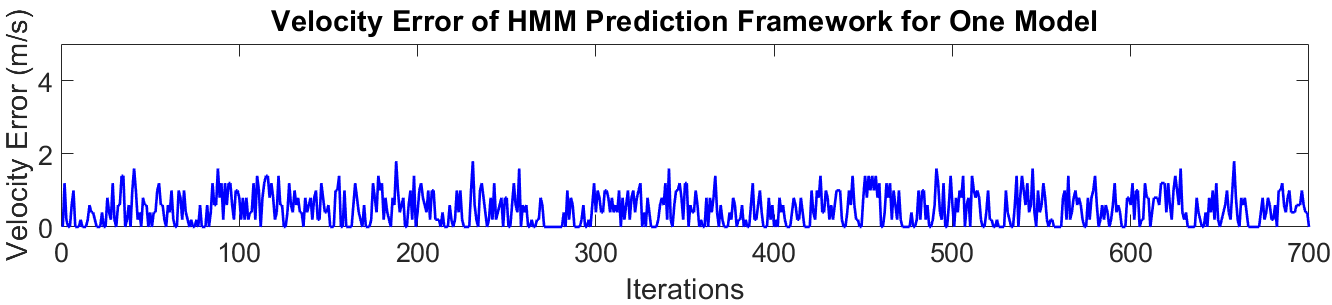
\includegraphics[width=0.48\textwidth]{fig/trainvelerror.png}
\caption{The error between the velocity of the actual model and estimated velocities} \label{fig:trainvel}
\end{figure}
\begin{figure}[ht]
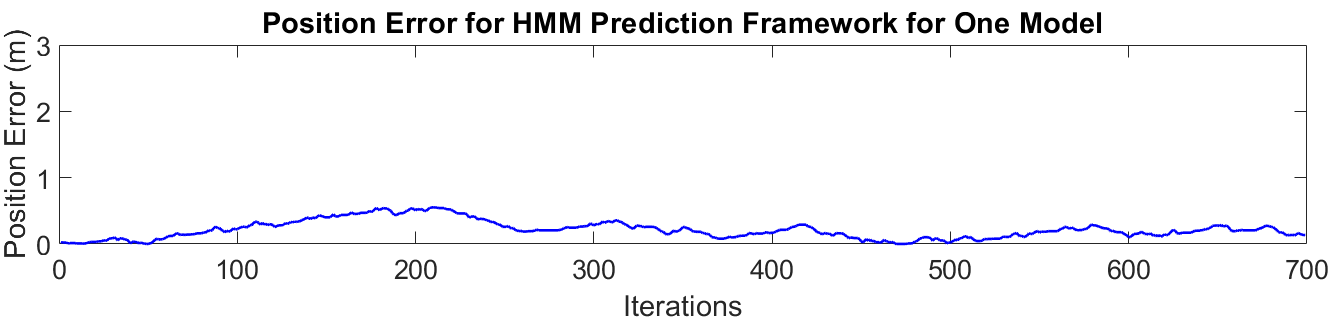
\includegraphics[width=0.48\textwidth]{fig/trainposerror.png}
\caption{The error between the position of the actual model and estimated positions} \label{fig:trainpos}
\end{figure}

In addition to velocity, we also measure the accuracy of our predictions regarding lane changes and following distances at which these changes occurred. Based on results shown in Fig.~\ref{fig:train2}, it is evident that the expected lane changes occurred, and to validate the following distances at which the lane changes took place, we used RMSE, which was $1.2564$m. The results for both velocity and lane change distance validation showed that the framework is very effective when predicting the future states of the same model.
\begin{figure}[ht]
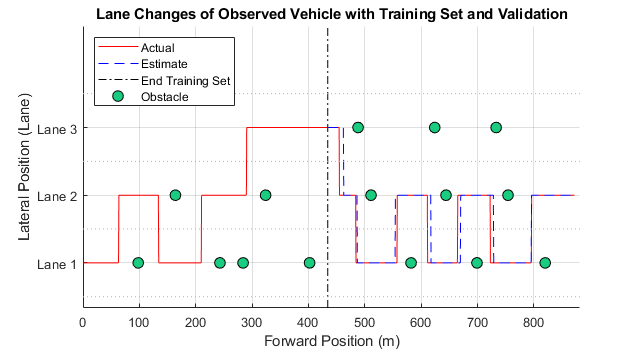
\includegraphics[width=0.48\textwidth]{fig/train2.png}
\caption{The lane changes of the actual vehicle and estimated vehicle} \label{fig:train2}
\end{figure}
\subsection{Fitting Models}
In this section, we add to the previous results, by showing that we are not only able to predict states given a model, but we are also able to fit pre-trained models to a new vehicle online. The behaviors of this vehicle are randomly generated and used to find the appropriate model. In order to determine the appropriate model, we initialize $\hat{\mathcal{P}}$ use \eqref{eq:pnorm} with the transition matrices of each of three pre-trained models. In Fig.~\ref{fig:error}, the error between each pre-trained model and the observed vehicle is shown. At the start of run-time, the errors are higher and are very scrambled. As the vehicle is observed for longer, one model has less error than the others; in this case, the model is Model $3$. 

\begin{figure}[ht]
    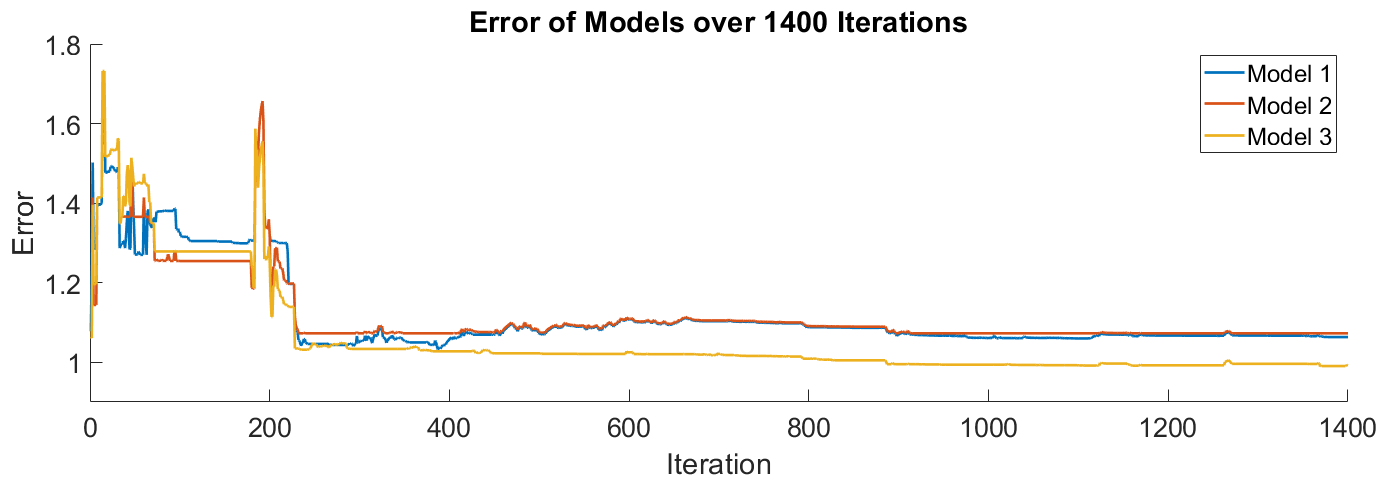
\includegraphics[width=0.48\textwidth]{fig/modelerror.png}
    \caption{The error of the fit between the current vehicle and each of the three pretrained models} \label{fig:error}
\end{figure}

At each iteration, we use the model with the lowest error for future predictions. The selected model changes frequently at the start of run-time and converges to one model by the end of run-time. The selected model at each iteration is shown in Fig.~\ref{fig:select}. In this case, we converge to Model $3$ in approximately 300 iterations.
\begin{figure}[ht]
    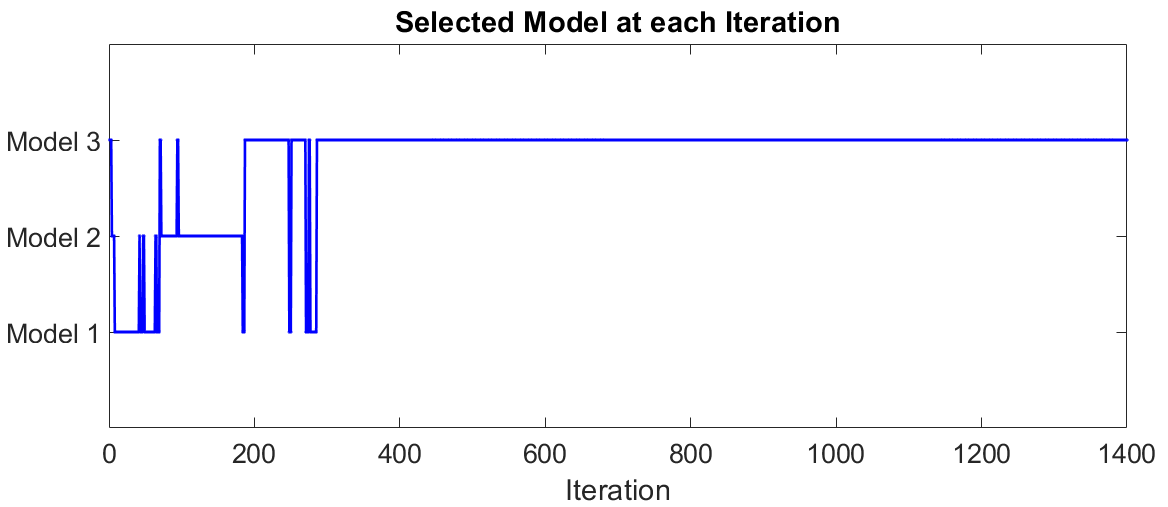
\includegraphics[width=0.48\textwidth]{fig/modelselect.png}
    \caption{The selected model at each iteration} \label{fig:select}
\end{figure}
Using the selected model, we are able to make predictions for every iteration of run-time. In Fig.~\ref{fig:fwd}, we show the accuracy of the fit for velocity/forward position over 1400 iterations. The RMSE of this trial was $2.1423$m/s. In Fig.~\ref{fig:lanchan}, we show the the predictions made that pertain to lane changes and following distance. The RMSE of the predictions as compared to the actual actions was $3.521$m. The RMSE values obtained for each of these tests suggest that the prediction is reliable, given that convergence to one model occurs. In addition, it was verified that the model chosen was the closest to the randomly generated behaviors, by examining the specific results of the randomization.

\begin{figure}[ht]
    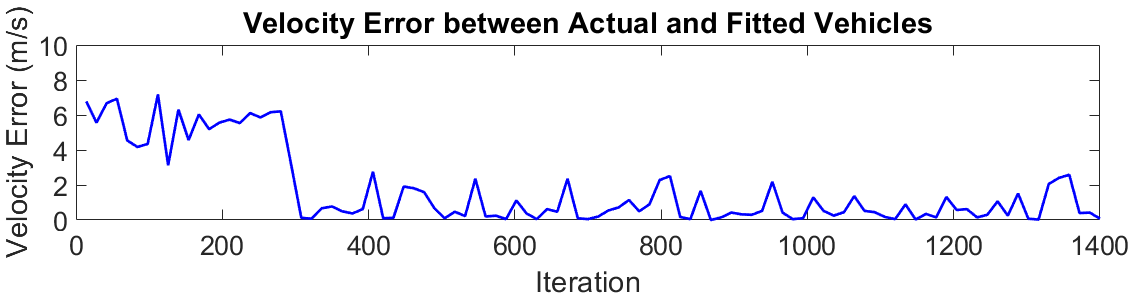
\includegraphics[width=0.48\textwidth]{fig/fiterroravg.png}
    \caption{Absolute Error of velocity between the fitted and actual vehicles} \label{fig:fwd}
\end{figure}

\begin{figure}[htpb!]
    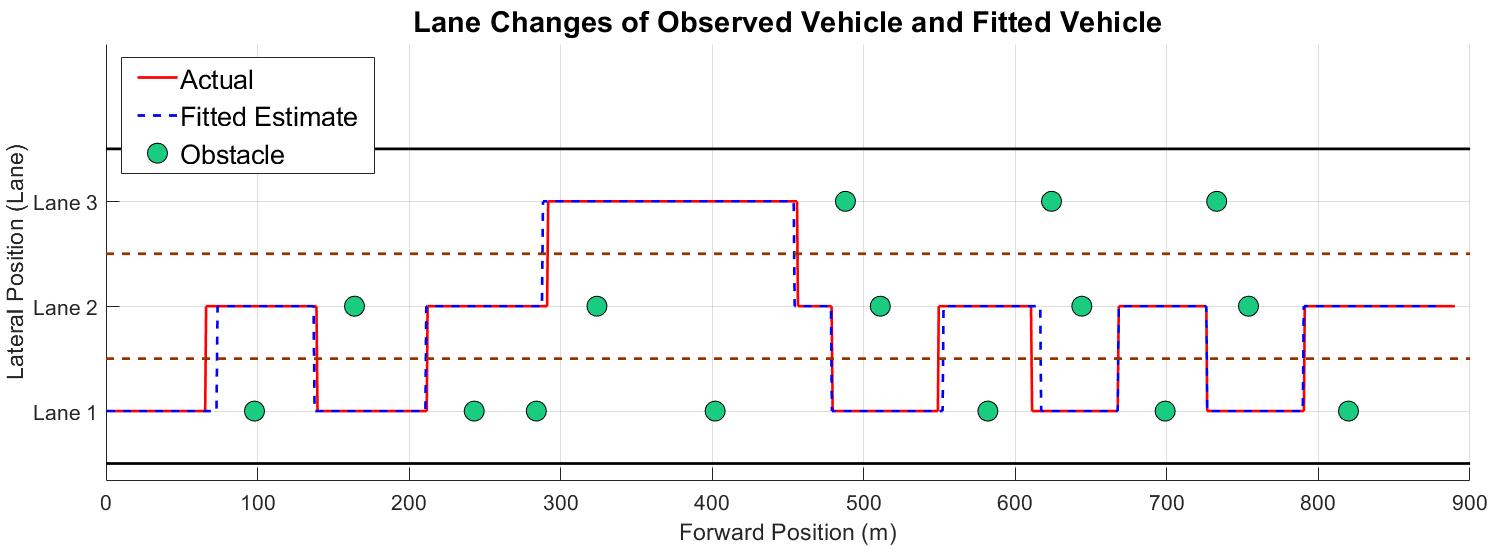
\includegraphics[width=0.48\textwidth]{fig/lanefit.png}
    \caption{The lane changes of the actual vehicle and the best-fit vehicle model} \label{fig:lanchan}
\end{figure}
\subsection{Assistive Planning and Control}
In order to show the impact of our assistive control, we simulate a scenario much like the one depicted in Fig.\ref{fig:hiway}. We show one case where the user has full control of the HAV, and one where assistance is given to the user. Depicted in Fig.~\ref{fig:critpt} is a scenario where the risk, $r_h\in\hat{\mathcal{R}}$ is nearing the user set limit of $r_{\max} = 0.85$.


\begin{figure}[h]
\centering
\begin{subfigure}{.54\linewidth}
  \centering
  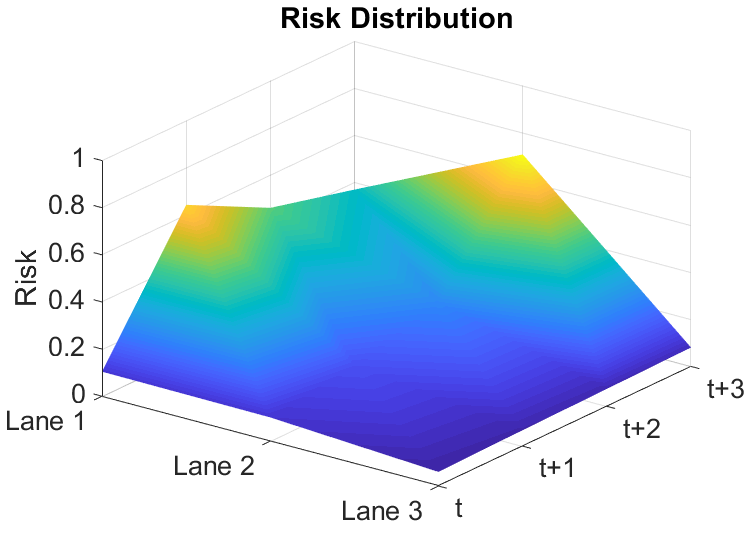
\includegraphics[width=\linewidth]{fig/critpt_rd.png}
  \caption{Risk Distribution}
  \label{fig:critptrd}
\end{subfigure}%
\begin{subfigure}{.46\linewidth}
  \centering
  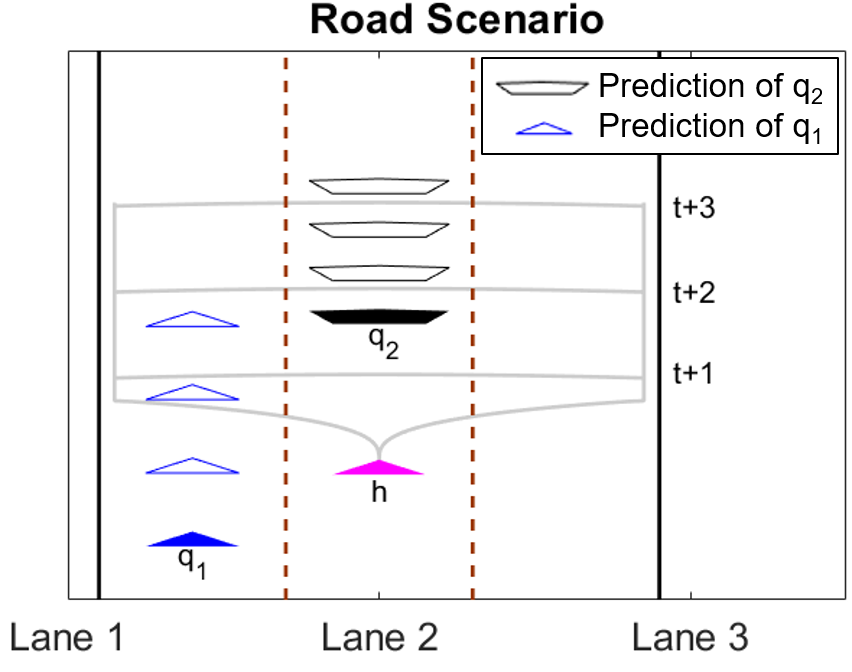
\includegraphics[width=\linewidth]{fig/critpt_rs.png}
  \caption{Road Scenario}
  \label{fig:critptrs}
\end{subfigure}
\caption{Critical Point - Risk Distribution and Road Scenario} \label{fig:critpt}
\end{figure}

In Fig.~\ref{fig:critpt}, the magenta vehicle in the center is the HAV we are able to control. The reachable set is shown coming out of the HAV, with the lines marked with $(t+1,t+2,t+3)$. In this case, we are only showing the reachable set and risk distribution for $v_h$. The situation depicted is one of a critical point, which means that a decision has to be made at this time, or there's a heightened chance a collision will occur within $H$. 


In Fig.~\ref{fig:noassist}, we show a scenario in which the user was unassisted. In this scenario, the user reached the same critical point as in Fig.~\ref{fig:critpt}, and decided to simply avoid vehicle $q_2$, by moving to the left lane, unaware that an increased risk exists in the future for the left lane. In addition, the user did not adjust their velocity either, and as a result a collision occurred.

\begin{figure}[h]
\centering
\begin{subfigure}{.54\linewidth}
  \centering
  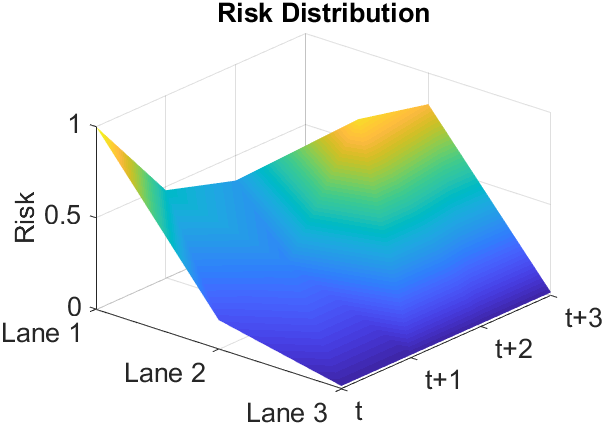
\includegraphics[width=\linewidth]{fig/noassist_rd.png}
  \caption{Risk Distribution}
  \label{fig:noasstrd}
\end{subfigure}%
\begin{subfigure}{.46\linewidth}
  \centering
  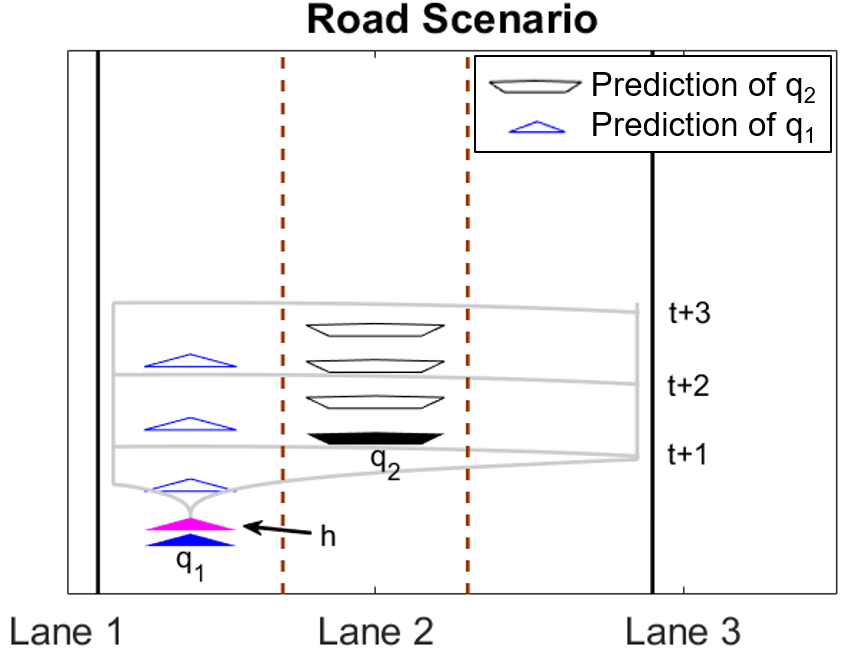
\includegraphics[width=\linewidth]{fig/noassist_rs.png}
  \caption{Road Scenario}
  \label{fig:noasstrs}
\end{subfigure}
\caption{Unassisted - Risk Distribution and Road Scenario} \label{fig:noassist}
\end{figure}

In our approach, we aim to avoid such a situation, and in Fig.~\ref{fig:assist}, we a show a scenario in which the HAV was assisted. The user input was modeled the same as in Fig.~\ref{fig:noassist}, but in this case, the assistive input was taken into account as the risk surpassed $r_{\max}$. With assistive input, both lane and velocity were changed in order to minimize risk. In this case, the specific input pair was $u_a = (l_3,v_h^+)$. 

\begin{figure}[h]
\centering
\begin{subfigure}{.54\linewidth}
  \centering
  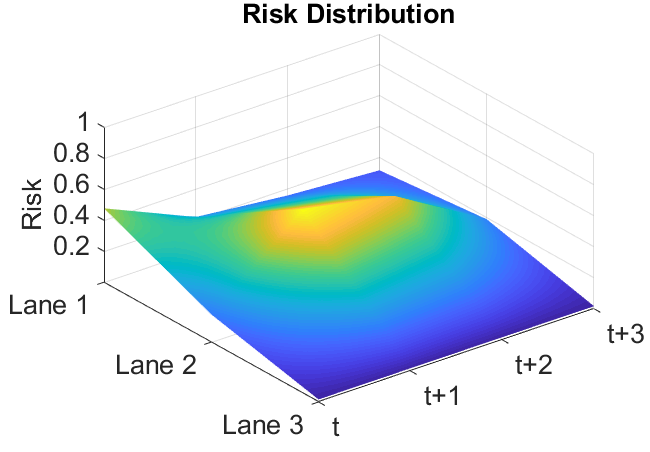
\includegraphics[width=\linewidth]{fig/assist_rd.png}
  \caption{Risk Distribution}
  \label{fig:assistrd}
\end{subfigure}%
\begin{subfigure}{.46\linewidth}
  \centering
  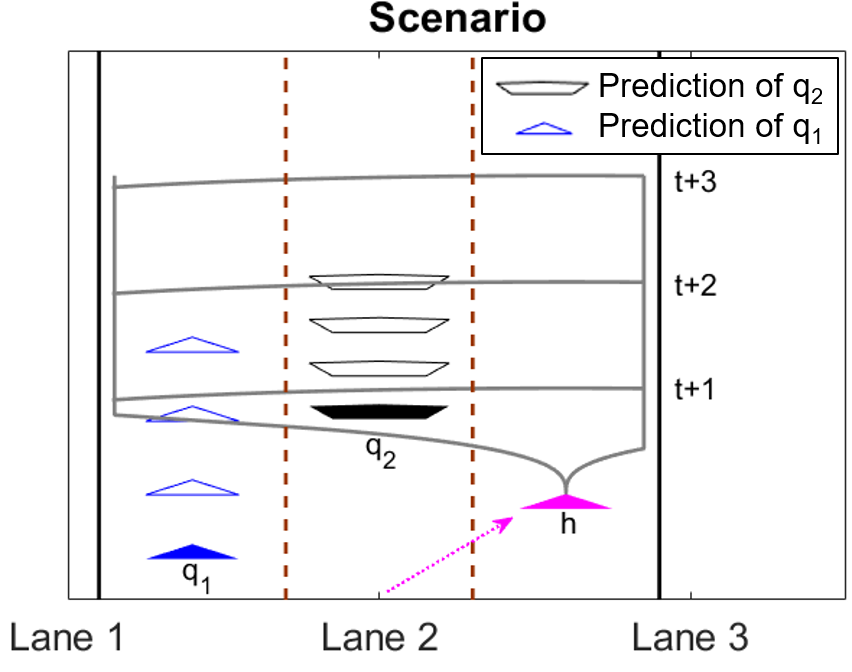
\includegraphics[width=\linewidth]{fig/assist_rs.png}
  \caption{Road Scenario}
  \label{fig:assistrs}
\end{subfigure}
\caption{Assisted - Risk Distribution and Road Scenario} \label{fig:assist}
\end{figure}

 In the situation depicted in Fig.~\ref{fig:assist}, the input $(l_3,v_h^+)$ increases the distance, $d_q(t)$, between vehicles $h$ and all $q$, which indicates risk has successfully been minimized for that timestep.


\section{Conclusions} \label{sec:concs}
%\NB{conclusions should summarize what we have accomplished with this work and what you learned from this work, including the pros and cons. They need to discuss also current and future directions.}
In this work, we have presented an approach for simultaneously predicting the future states of multiple vehicles and assisting the user of an HAV. Our approach uses a Hidden Markov Model based framework to build offline models of different vehicles and fit these models to any number of online observed vehicles. A shared control scheme was also presented to ensure that the user of an HAV does not enter an unsafe state. We were able to show that by minimizing our predicted risk at each step, we are able to ensure the vehicle stays as safe as possible. While the prediction method is reliable, model fitting is most effective when the set of offline models is rich and varied enough such that any vehicle can be fitted accurately.

In future work, we will build more pre-trained models to increase richness. In this work, we are primarily concerned with the technique, but plan to expand the prediction framework to a more realistic situation, involving more realistic dynamics and other factors, such as external disturbances. In addition, we plan to expand our framework across different types of vehicles and other cyber-physical systems.

\section{Acknowledgement}

%\NB{KEEP THIS - this sentence needs more explanation. If we don't have enough models we need to mention that future work is centered on using existing models to extract new models}
% references section

% can use a bibliography generated by BibTeX as a .bbl file
% BibTeX documentation can be easily obtained at:
% http://mirror.ctan.org/biblio/bibtex/contrib/doc/
% The IEEEtran BibTeX style support page is at:
% http://www.michaelshell.org/tex/ieeetran/bibtex/
%\bibliographystyle{IEEEtran}
% argument is your BibTeX string definitions and bibliography database(s)
%\bibliography{IEEEabrv,../bib/paper}
%
% <OR> manually copy in the resultant .bbl file
% set second argument of \begin to the number of references
% (used to reserve space for the reference number labels box)

%\begin{thebibliography}{1}

%\bibitem{IEEEhowto:kopka}
%H.~Kopka and P.~W. Daly, \emph{A Guide to \LaTeX}, 3rd~ed.\hskip 1em %plus
%  0.5em minus 0.4em\relax Harlow, England: Addison-Wesley, 1999.
  
  
%\end{thebibliography}

%\printbibliography
\bibliographystyle{abbrv}
\bibliography{mybibliography.bib}


% that's all folks
\end{document}


